\documentclass{sigchi}




% Use this section to set the ACM copyright statement (e.g. for
% preprints).  Consult the conference website for the camera-ready
% copyright statement.

% Copyright
%\CopyrightYear{2018}
%\setcopyright{acmcopyright}
%\setcopyright{acmlicensed}
%\setcopyright{rightsretained}
%\setcopyright{usgov}
%\setcopyright{usgovmixed}
%\setcopyright{cagov}
%\setcopyright{cagovmixed}
% DOI
\doi{http://dx.doi.org/10.475/123_4}
% ISBN
\isbn{123-4567-24-567/08/06}
%Conference
%\conferenceinfo{CHI'18,}{April 21--26, 2018, Montr\'{e}al, Canada}
\conferenceinfo{}{Submitted for review to ACM CHI 2018. Do not distribute.}
%Price
%\acmPrice{\$15.00}

% Use this command to override the default ACM copyright statement
% (e.g. for preprints).  Consult the conference website for the
% camera-ready copyright statement.

%% HOW TO OVERRIDE THE DEFAULT COPYRIGHT STRIP --
%% Please note you need to make sure the copy for your specific
%% license is used here!
% \toappear{
% Permission to make digital or hard copies of all or part of this work
% for personal or classroom use is granted without fee provided that
% copies are not made or distributed for profit or commercial advantage
% and that copies bear this notice and the full citation on the first
% page. Copyrights for components of this work owned by others than ACM
% must be honored. Abstracting with credit is permitted. To copy
% otherwise, or republish, to post on servers or to redistribute to
% lists, requires prior specific permission and/or a fee. Request
% permissions from \href{mailto:Permissions@acm.org}{Permissions@acm.org}. \\
% \emph{CHI '16},  May 07--12, 2016, San Jose, CA, USA \\
% ACM xxx-x-xxxx-xxxx-x/xx/xx\ldots \$15.00 \\
% DOI: \url{http://dx.doi.org/xx.xxxx/xxxxxxx.xxxxxxx}
% }

% Arabic page numbers for submission.  Remove this line to eliminate
% page numbers for the camera ready copy
\pagenumbering{arabic}

% Load basic packages
\usepackage{balance}       % to better equalize the last page
\usepackage{graphics}      % for EPS, load graphicx instead 
\usepackage[T1]{fontenc}   % for umlauts and other diaeresis
\usepackage{txfonts}
\usepackage{mathptmx}
\usepackage[pdflang={en-US},pdftex]{hyperref}
\usepackage{color}
\usepackage{booktabs}
\usepackage{textcomp}

% Some optional stuff you might like/need.
\usepackage{microtype}        % Improved Tracking and Kerning
% \usepackage[all]{hypcap}    % Fixes bug in hyperref caption linking
\usepackage{ccicons}          % Cite your images correctly!
% \usepackage[utf8]{inputenc} % for a UTF8 editor only

% If you want to use todo notes, marginpars etc. during creation of
% your draft document, you have to enable the "chi_draft" option for
% the document class. To do this, change the very first line to:
% "\documentclass[chi_draft]{sigchi}". You can then place todo notes
% by using the "\todo{...}"  command. Make sure to disable the draft
% option again before submitting your final document.
\usepackage{todonotes}

% Paper metadata (use plain text, for PDF inclusion and later
% re-using, if desired).  Use \emtpyauthor when submitting for review
% so you remain anonymous.
\def\plaintitle{Sketch\&Stitch: Interactive Embroidery for E-Textiles}
\def\plainauthor{First Author, Second Author, Third Author,
  Fourth Author, Fifth Author, Sixth Author}
\def\emptyauthor{}
\def\plainkeywords{E-textile; interactive fabrication; embroidery; sketching}
\def\plaingeneralterms{Documentation, Standardization}

% llt: Define a global style for URLs, rather that the default one
\makeatletter
\def\url@leostyle{%
  \@ifundefined{selectfont}{
    \def\UrlFont{\sf}
  }{
    \def\UrlFont{\small\bf\ttfamily}
  }}
\makeatother
\urlstyle{leo}

% To make various LaTeX processors do the right thing with page size.



\def\pprw{8.5in}
\def\pprh{11in}
\special{papersize=\pprw,\pprh}
\setlength{\paperwidth}{\pprw}
\setlength{\paperheight}{\pprh}
\setlength{\pdfpagewidth}{\pprw}
\setlength{\pdfpageheight}{\pprh}

\usepackage{draftwatermark}
\SetWatermarkText{\parbox{50cm}{\centering%
  Author's Copy \\
  Submitted to CHI'18 \\
  Do not distribute}}
\SetWatermarkScale{.5}

% Make sure hyperref comes last of your loaded packages, to give it a
% fighting chance of not being over-written, since its job is to
% redefine many LaTeX commands.
\definecolor{linkColor}{RGB}{6,125,233}
\hypersetup{%
  pdftitle={\plaintitle},
% Use \plainauthor for final version.
%  pdfauthor={\plainauthor},
  pdfauthor={\emptyauthor},
  pdfkeywords={\plainkeywords},
  pdfdisplaydoctitle=true, % For Accessibility
  bookmarksnumbered,
  pdfstartview={FitH},
  colorlinks,
  citecolor=black,
  filecolor=black,
  linkcolor=black,
  urlcolor=linkColor,
  breaklinks=true,
  hypertexnames=false
}

% create a shortcut to typeset table headings
% \newcommand\tabhead[1]{\small\textbf{#1}}

% End of preamble. Here it comes the document.


\usepackage{subfiles}

\newcommand\nur[1]{\textcolor{blue}{#1}}


\begin{document}
\title{\plaintitle}

\numberofauthors{1}
\author{
  Nur Al-huda Hamdan \hspace*{0.9cm} Simon Voelker \hspace*{0.9cm} Jan Borchers\\
  \\
    \affaddr{RWTH Aachen University}\\
    \affaddr{52074 Aachen, Germany}\\
    \email{\{hamdan, voelker, borchers\}@cs.rwth-aachen.de}
}




\teaser{
%\begin{figure}
\centering
\includegraphics[width=1\textwidth]{figures/Fig1_Nur}
\caption{Sketch\&Stitch walkthrough: (a) A user sketches artwork directly on fabric, (b) she uses \textit{Circuit Stickers} to plan the circuit layout, (c) she draws circuit traces to connect the stickers, (d) the system takes a picture of the sketch, converts it into embroidery patterns, and sends them to an embroidery machine for stitching using conductive and non-conductive threads, (e) the user replaces Circuit Stickers with real electrical components and attaches them to the fabric.
}
 \vspace{-1em}
\label{fig:Fig1}
}

\maketitle



\begin{abstract}
E-Textiles are fabrics that integrate electronic circuits and components. Makers use them to create interactive clothing, furniture, and toys. However, this requires significant manual labor and skills, and using technology-centric design tools. We introduce \textit{Sketch\&Stitch}, an interactive embroidery system to create e-textiles using a traditional crafting approach: Users draw their art and circuit directly on fabric using colored markers. The system takes a picture of the sketch, converts it into embroidery patterns, and sends them to an embroidery machine. Alternating between sketching and stitching, users build and test their design incrementally. Sketch\&Stitch features \textit{Circuit Stickers} representing circuit boards, components, wire crossings to insulate, and various textile touch sensors such as pushbuttons, sliders, and 2D touchpads. Circuit Stickers serve as placeholders during design. Using computer vision, they are recognized and replaced later in the appropriate embroidery phases. We close with technical considerations and application examples.
\end{abstract}


\category{H.5.2}{User Interfaces}{}

\keywords{\plainkeywords}

\section{Introduction}


Electronic textile technology enables people to create expressive, interactive, and functional textile artifacts for both playful and serious applications.
It combines the visual and haptic expressiveness of textiles with the interactivity and utility of electronic components such as LEDs, vibration motors, speakers, GPS receivers, and touch sensors. At the intersection of technology, art, and fashion (see, e.g., CuteCircuit.com), e-textiles have attracted artists, designers, hobbyists, and makers applying this technology in creative and artistic ways \cite{berzowska2005kukkia,Buechley:2010:LWH:1858171.1858206}. 
%Other e-fashion companies:
%https://iq.intel.com/fashion-metamorphosis-meet-the-butterfly-dress/
%http://ezratuba.com/wearable-tech
%Berlin University of the Arts - Department of Textile and Surface Design
This has motivated HCI research to investigate techniques that enable a wider audience to integrate fabrics and electronics into interactive textiles \cite{Buechley2009,perner2011handcrafting,5387040}.

In e-textiles, conductive threads, inks, polymers, or textiles are attached directly to a base fabric, creating \textit{fabric circuits}. These circuits connect traditional electronic components, usually on printed circuit boards, but they can also directly include functional parts such as fabric-based resistors, capacitors, touch sensors, actuators \cite{stylios2007shape}, or antennas \cite{catrysse2004towards}.
%batteries \cite{}
%powering elements \cite{}
Creating e-textiles typically involves 1.\ designing or choosing an artwork, 2.\ planning the layout of electrical components and traces, 3.\ creating the artwork and fabric circuit on the base fabric, 4.\ insulating circuit traces where necessary, and 5.\ attaching electronic components \cite{Lovell:2010:ETD:1810543.1810578}. 
The techniques for implementing e-textiles are based on traditional methods such as weaving \cite{kallmayer2003new}, embroidery \cite{5387040}, and printing \cite{kim2010electrical}.
%\cite{castano2014smart,mattila2006intelligent}. These citations provide a review of methods

%Some of these techniques have been successfully adopted by the do-it-yourself community 
% as evident from makers' websites, such as Instructables\footnote{https://www.instructables.com/}, Sparkfun\footnote{https://www.sparkfun.com/} and Adafruit\footnote{https://www.adafruit.com/}. But these techniques have some constraints.
%More websites: https://www.lib.ncsu.edu/softcircuits


As users rely predominantly on manual implementation of e-textiles \cite{Kazemitabaar:2017:MTA:3025453.3025887}, executing a design becomes labor-intensive and requires high skill levels as the number and density of electrical components and connections increase. Debugging e-textiles is only possible after investing considerable time in building them. Insulating circuit traces is an extra step requiring special tools and materials \cite{Buechley2009}. Observing participants in our e-textile workshops, and analyzing over 70 e-textile projects documented online, we found that this laborious multi-step process often forced them into trade-offs between the visual and functional aspects of their design, impeding improvisation and exploration. The lack of a design pipeline and digital support for e-textile fabrication can thus limit the creative and iterative design of e-textiles.
%enable users to focus and invest their time on the visual and functional aspects of their project.

% We analysed more than 70 e-textile projects on the mentioned websites and found that makers make a trade-off between the fidelity of the artistic pattern and the functionality of the artefact. 


In this paper, we present \emph{Sketch\&Stitch,} an interactive embroidery system that enables users to create e-textiles by sketching on fabric (Fig.~\ref{fig:Fig1}). It uses a computerized embroidery machine as a digital fabrication tool to handle the two most laborious steps when creating e-textiles, stitching and insulation. Sketch\&Stitch features \textit{Circuit Stickers}, printed adhesives representing elements users can embed into their design, from circuit boards and components, to wire crossings to insulate, to various textile touch sensors. These stickers guide the user while drawing circuit traces to ensure reliable electrical connections, and are recognized using computer vision, automatically generating stitching patterns for sensors, insulations, and wire crossings, for example.

% In Sketch\&Stitch, a user begins by sketching an artwork on the workpiece fabric using colored fabric markers. She plans the placement of components using Circuit Stickers and draws connections. When she is ready to execute the design, the system takes a picture of the sketch, converts it into embroidery patterns, and sends them to an embroidery machine. 
% %The embroidery machine's embedded display allows the user to verify the patterns and make minor adjustments before stitching is started. 
% The user may repeat these steps to review and test parts of her art and circuitry incrementally. Some Circuit Stickers, e.g., for touch sensors, are already replaced with stitches automatically by the system. After embroidery is complete, the user replaces the remaining Circuit Stickers with their component counterparts, using one of three attachment techniques we describe.

In the remainder of this paper, after reviewing related work, we first briefly introduce the reader to the particular features of computerized embroidery machines that are relevant for this work. We present Sketch\&Stitch and its interaction design. We illustrate the extensions we added to Sketch\&Stitch beyond the basic system that enable a wider range of practical applications, and walk the reader through a concrete example. After providing details on the software implementation and recommendations for materials and stitching techniques, we present several example artifacts created using our system, and close by discussing the current limitations of Sketch\&Stitch and opportunities for future research.

In summary, this paper makes the following contributions:
\begin{itemize}
    \item Sketch\&Stitch, a new approach and system prototype to create e-textiles by drawing directly on the fabric;
    \item Interaction techniques and embroidery patterns that let users include circuit boards, components, insulation, wire crossings, and a variety of fabric sensors using Circuit Stickers;
    \item Technical recommendations for materials and stitching processes to create e-textiles with digital embroidery machines.
\end{itemize}


% Machine embroidery has bloomed entering homes, makerspaces and design studios of crafters, hobbyists and DIY.

% \url{http://www.strategyr.com/MarketResearch/Sewing_Machines_Market_Trends.asp}

% \url{http://robyns.world/2015/06/13/infographic-sewing-machine-day/}


\subfile{RelatedWork}

\section{Embroidery Machines In Personal Fabrication}
Computerized embroidery machines became available to homes and small business in the 1980s. At prices between 500 and 15,000 US Dollars, they have become a tool frequently found in schools, maker spaces, and small businesses \cite{lipson2010factory}, and are part of the MIT recommended Fab Lab inventory\footnote{fab.cba.mit.edu/about/fab/inv.html}, for example.
Embroidery machines use a hoop system to hold the framed area of fabric taut under the needle and move it automatically along the $x$ and $y$ axes to stitch embroidery patterns. A presser foot, a metallic attachment that surrounds the needle, holds the fabric flat during embroidery to prevent it from rising and falling with the needle. A control panel and embedded display provide basic functionality to, e.g., start/stop the machine, control thread tension, change stitching speed, view embroidery patterns and make minor adjustments such as re-positioning, scaling, rotating, mirroring, and re-ordering. Home embroidery machines can stitch up to 1000 stitch/min.


 \begin{figure}
\centering
  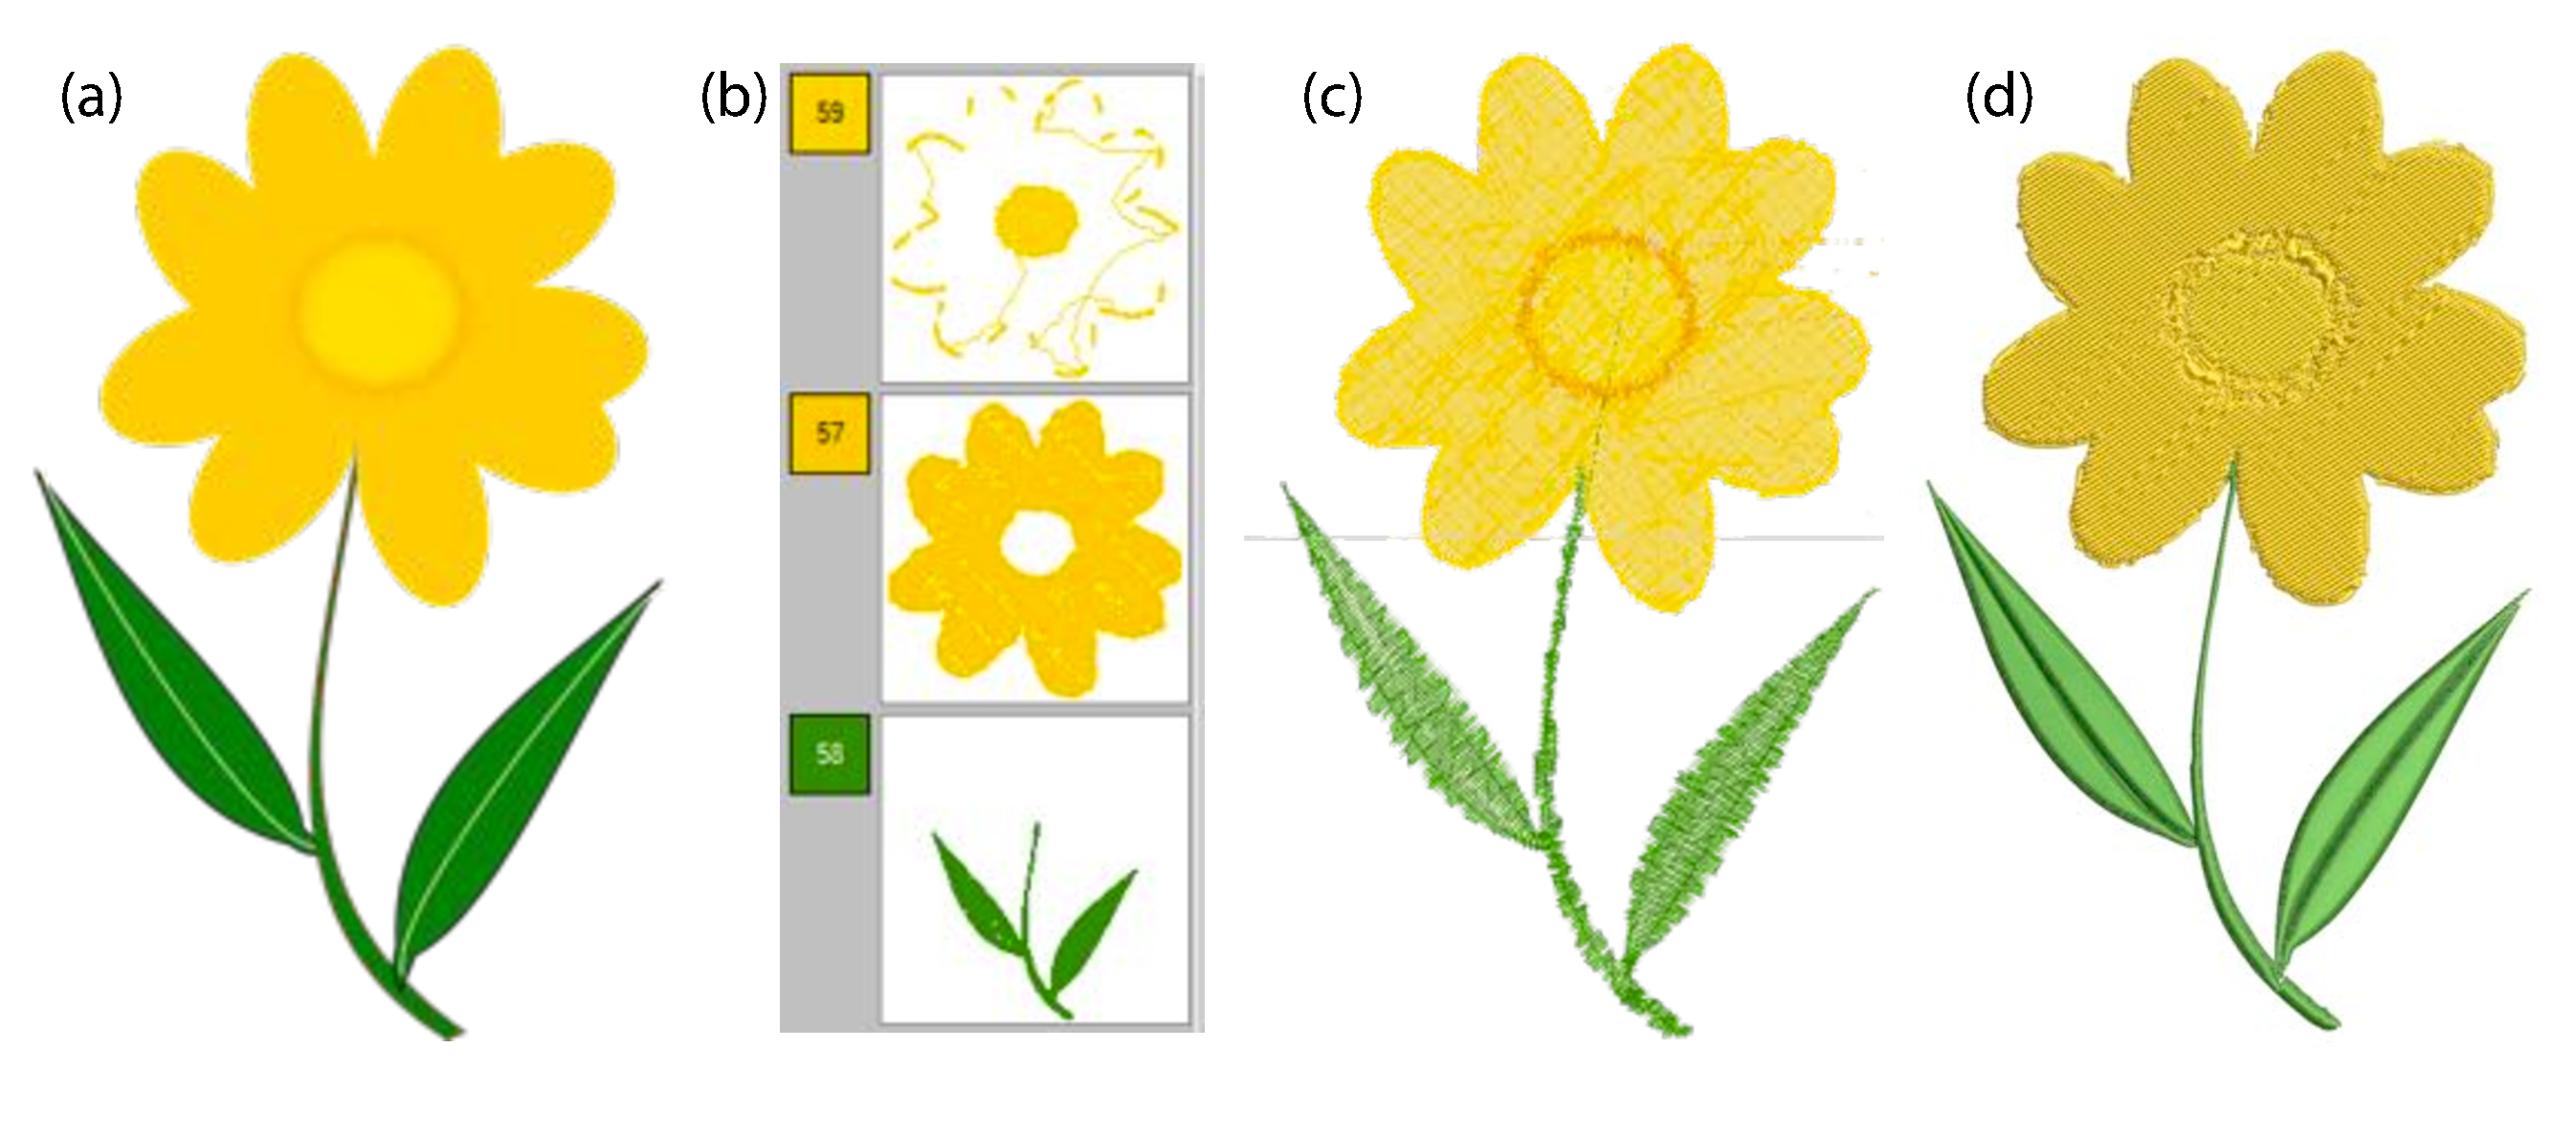
\includegraphics[width=0.9\columnwidth]{figures/EMWorkflow}
  \caption{Image digitization in embroidery software: (a) imported image, (b) separation into color layers with assigned thread colors, (c) generated tool path, (d) final embroidery pattern }~\label{fig:EmbroideryWorkflow}
  \vspace{-2.5em}
\end{figure}

Embroidery machines come with proprietary software that runs on the user's computer. The software transforms color images into embroidery patterns and generates a tool path for the machine. The path dictates how an embroidery hoop moves under the needle. It includes stitch patterns, thread color changes, and jump stitches when traveling between different stitch objects. To optimize tool path generation, embroidery software separates design objects into multiple layers based on color (Fig.\ \ref{fig:EmbroideryWorkflow}). That way, the machine has to stop and prompt the user to manually change thread color less often. Jump stitches also need to be trimmed by hand after embroidery. To reduce these jumps, professional embroidery designers often re-program patterns, manually sequencing stitch objects and individual stitches. 
%Industrial embroidery machines can change thread colors automatically. 
An embroidery machine reads a digitized embroidery pattern from a memory card or a computer connection, recognizes color layers, and stitches them sequentially.

%Virtual hoops help the user position, orient and scale a design relative to physical hoops. 
%Some software tools allow the user to print a design inside a virtual hoop in life-scale to assist the user in aligning the physical hoop on the workpiece fabric.

The internal algorithms that generate a concrete stitching pattern and tool path from a design encode advanced expertise in the mechanical properties of fabrics and threads, not unlike the slicing software turning 3D models into print head tool paths for 3D printers. This complexity is usually kept from the user, but embroidery software still has a relatively steep learning curve, offering a large number of visual design options and specialized tools for manipulating stitch patterns, such as a parametric stitch designer and pull compensation options.
Its user interface assumes a nontrivial amount of expertise in threads, fabrics, embroidery, and the workings of the machine.

\section{Sketch\&Stitch}
Sketch\&Stitch utilizes an embroidery machine to take over the laborious tasks in e-textile fabrication---stitching and insulating conductive traces. Yet, it maintains the physical and direct interaction between the user and the fabric work piece during the creative tasks---designing and planning visual and functional patterns. 
%By this, the system aims to ... 
%reduce the entry barrier to e-textile fabrication and 
%encourage creative and improvisational and creative designs.

The Sketch\&Stitch system comprises a commercial embroidery machine, a computer, a smartphone on a camera mount above the work surface, and a Bluetooth-connected button to trigger the capture process. Smartphone runs our app for color calibration and image capture. The computer runs the manufacturer's proprietary embroidery software, and our Sketch\&Stitch software for image processing and communicating with that software as well as the machine itself.

The workflow with Sketch\&Stitch was developed with designers and makers in mind. %and artists
It enables them to convert an idea sketched on fabric into an interactive embroidery without having to interact with computer screens or CAD/CAM tools. Unlike circuit layout software such as Fritzing or Autodesk's Eagle, Sketch\&Stitch lets users draw both artwork and electrical connections in free artistic shapes directly on the fabric, allowing sketching and drawing aesthetics to shape the overall design. 
%Physical sketching provides users with continuous representation of their workpiece and helps them establish a closer relation with the materials (fabrics, threads, electronics) to better understand their properties and nuances \cite{willis2011interactive}. 
Users interact with Sketch\&Stitch using colored fabric markers and \textit{Circuit Stickers}. It is thus designed for improvisational design and quick, low-threshold prototyping.
 
%Potentially, it can lowers the barrier for designing e-textiles
%feedback on how a design (i.e., position, orientation, scale) will appear

%asses the visual design, test circuit layouts, or evaluate how the fabric material will behave when electrical components are attached to it
%It automizes the digitization of designs into embroidery patterns, and includes new patterns for conductive thread. 


Circuit Stickers are symbolic images printed on adhesive paper. %They have the same shape, size and name of circuit elements they represent.
They represent elements to be added to the fabric circuit during and after embroidery. Circuit Stickers were developed for two reasons: First, the presser foot in embroidery machines only has a clearance of about 1 mm above the fabric, too low for even thin populated PCBs. This leads to the risk of breaking the needle or machine if they come in contact. Second, we wanted to save the user having to hand-draw the multi-layer embroidery patterns our textile touch sensors etc.\ require.

Sketch\&Stitch supports two types of Circuit Stickers: \emph{Component Stickers} and \emph{Embroidery Stickers}. Component Stickers address the first problem above. They serve as placeholders for electronic components such as LEDs, motors and speakers, usually on PCBs. Users replace them with their hardware counterparts after embroidery is complete, using one of three attachment techniques we describe further below.

Embroidery Stickers represent multi-layer custom embroidery patterns required for insulated traces, wire crossings, and our various textile touch sensors.
The user removes these stickers after capturing their design via the camera, and our system inserts the required multi-layer patterns in place automatically during the embroidering process.

Both kinds of Circuit Stickers help users plan and sketch a circuit with ease and precision. Their adhesive backing allows the user to experiment with different positions  during the design phase, and holds them in place while the fabric is being moved around.
%Some stickers include grooves to guide users' traces to ensure reliable electrical connection with the added units. 
The resulting end-to-end workflow of Sketch\&Stitch is to 1.\ sketch an artwork directly on fabric with a textile marker, 2.\ plan and place Circuit Stickers and draw connections between them, 3.\ capture the design via a camera, 4.\ remove any Embroidery Stickers and stitch the design on the embroidery machine, and finally 5.\ attach the electronics, replacing any Component Stickers. We look at these steps and our solutions for advanced features below.

%  We aim to make e-textile creation accessible for emerging designers, hobbyists, crafters, and makers.
%To keep the traditional craft ways of entirely working on the physical workpiece, we developed a pipeline that enables users to sketch the design and plan the circuit directly on fabric. This pipeline 
% Simulating the traditional craft ways of directly interacting with the physical form using tools opens up a range of new creative possibilities [].
%Disconnect between physical and digital: There are numerous sources of variability in textile materials that can make a digital representation unstable, regardless of how good the simulation is.
% More agency and control over the final outcome [Being the Machine: Reconfiguring Agency and Control in Hybrid Fabrication].




\subsection{Sketching the Design}
Drawing on fabric is an established art form, and used to design patterns for manual embroidery. 
Sketch\&Stitch uses simple markers, enabling users to express themselves freely without the constraints of design applications \cite{landay1995interactive,schweikardt2000digital}. The markers use water-soluble inks and can be washed out later.

To start sketching on fabric, a user secures it in an embroidery hoop of the desired size. The hoop holds the fabric flat and taut, and frames the design location on the work piece. Next, she selects her marker color palette and follows color calibration instructions on the Sketch\&Stitch mobile app: Using a printable calibration template, the user indicates a \textit{trace color} for drawing electrical traces, an optional \textit{insulation color} if needed, and up to six \textit{art colors} for drawing the artwork (these are usually not the final \emph{thread colors}, see below).
The system preserves three distinct colors for Circuit Stickers. To be able to extend a partly stitched design in subsequent iterations, the user should avoid using thread colors that appear in her marker color palette. Sketch\&Stitch uses colors instead of symbolic sketch annotations for user-system communication to avoid imposing design constraints on freehand sketches, and to keep the design uncluttered. In addition, Sketch\&Stitch uses colors to enforce the sequence of pattern execution when communicating with the embroidery software. For example, in a simple design, the system sequences all objects in \texit{trace color} to be stitched first using conductive thread, followed by objects in each \textit{art color} using non-conductive threads.


 
The user can draw their art and circuit in any order.
%When drawing circuit traces, the user should keep using the trace color marker from the calibration process. 
To \textit{undo} any markings, she erases marker strokes by patting on the fabric with a damp cloth. The amount of detail the system can recognize in a design depends mainly on the quality of the image captured (camera, lighting), fabric texture, and marker quality (tip and color consistency). 

A design does not need to be complete before it can be stitched. At any point, the user can take a picture of the fabric, secure the hoop in the embroidery machine, and start the stitching process. This enables her to evaluate and test her design early on, supporting \textit{incremental design}. To continue sketching on an already embroidered fabric, she first captures a picture of the current embroidered state before proceeding.

\subsection{Adding Electronics}
The user places Component Stickers on the fabric to serve as placeholders for the electronics hardware to embed in the design. As illustrated above, embroidering with hardware components on the fabric is very challenging for most embroidery machines due to the low \textasciitilde 1 mm clearance of the presser foot. For comparison, LilyPad PCBs are .8 mm thick, but more than 2 mm high when including their SMD components.

Figure \ref{fig:ComponentStickers} shows sample stickers for the LilyPad kit. Stickers have the same shape, size, and name of their physical counterparts.  
The grooves near the pin holes are added to guide the user and ensure that circuit traces extend under the component and create sufficient contact surface for the attached board. 
%LilyPad components have exposed conductive plates on the top and bottom of the PCB.
The user prints these stickers from the Sketch\&Stitch mobile app on adhesive paper using any printer. Stickers are tinted with two \textit{sticker colors} (here, black and white). To use a sticker, she cuts it out, peels off the backing, and adheres it to the fabric. %\emph{Embroidery Stickers} representing touch sensor areas can be cut to any desired size. 
Using the \textit{trace color} marker, she then draws circuit traces to connect the sticker. 
%The user may use a vinyl cutter to quickly cut them into shape. 
Circuit Stickers can be created for any PCBs or off-the-shelf components. The only constraint is that they must have a pitch of 2.5 mm or wider between their leads (we discuss this in section Technical Considerations). Circuit Stickers can be reused in later projects.


\begin{figure}
\centering
  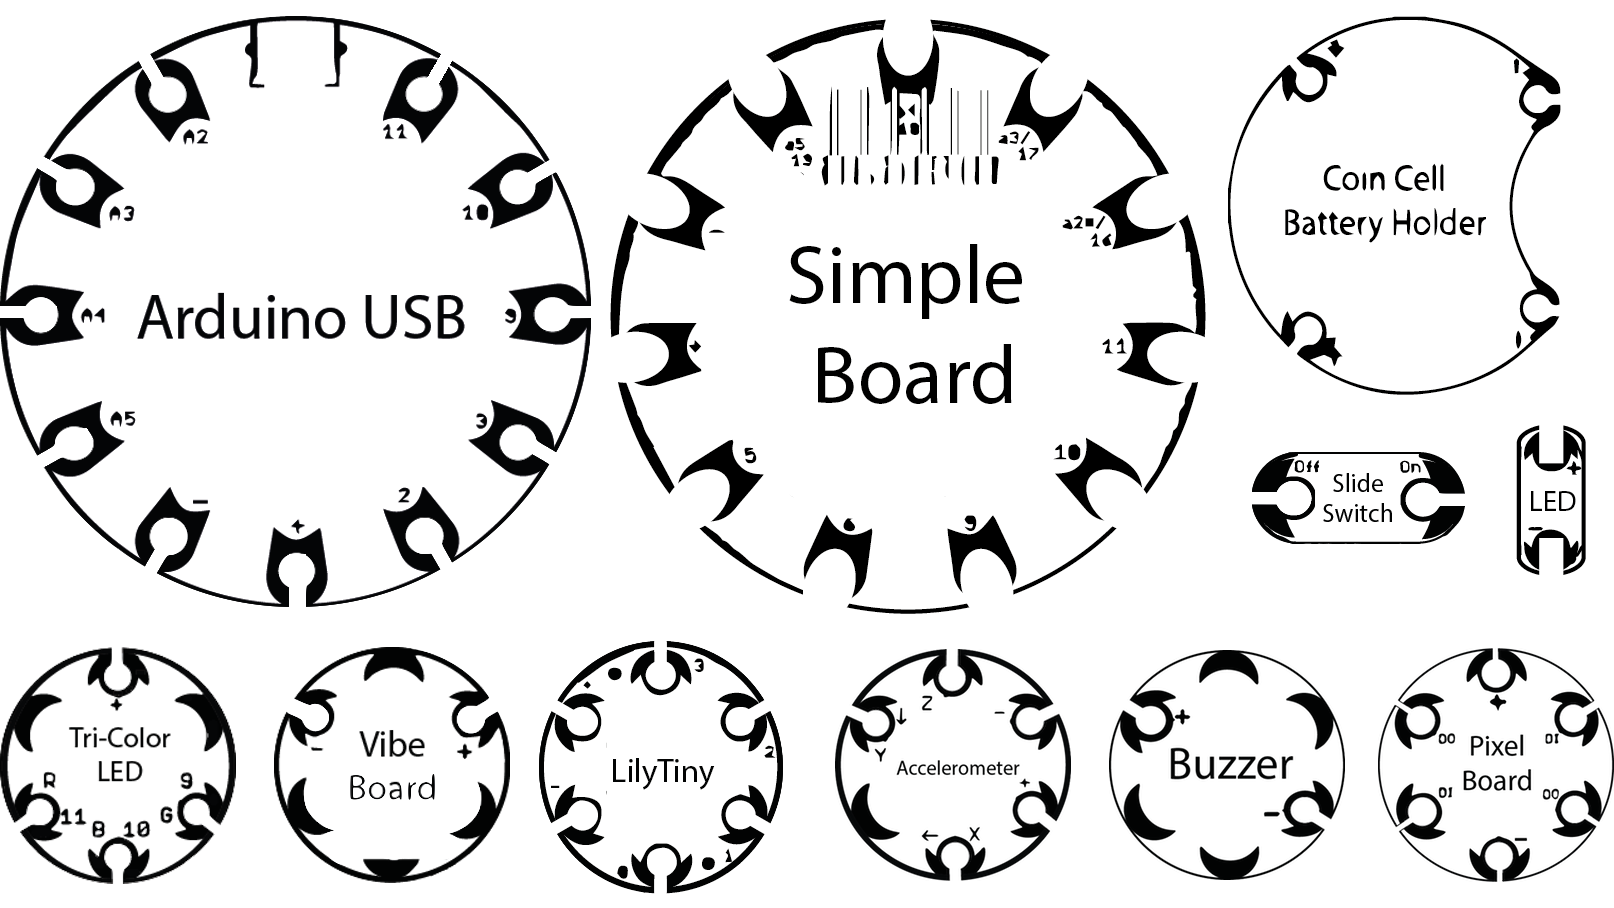
\includegraphics[width=0.9\columnwidth]{figures/ComponentStickers.png}
  \caption{Component Stickers for the Arduino LilyPad electronics kit.}~\label{fig:ComponentStickers}
  \vspace{-1.5em}
\end{figure}

\subsection{Attaching Electronics}
%We mainly considered sewable components, and components with flat pads on the wrong side of the unit.




After embroidery is complete, the user replaces all Component Stickers with their corresponding hardware components and attaches them to the fabric.
%Sketch\&Stitch simplifies this step by stitching the contact surface  d. 
%Attaching hardware circuit boards and components to fabric is one of the main challenges in e-textiles. Researches have explored several techniques including soldering [], special soldering [], manual sewing [], breads [], ...
We describe three techniques for attaching electronics to fabric. The first uses 3M Z-tape, a double-sided adhesive that conducts in the $z$ dimension only when compressed. A piece of Z-tape is applied to the back of a component, and the component is aligned to the stitched contact surface on the fabric. Pressing the component down onto the fabric creates connections between pins and contact areas through the Z-Tape. This technique is especially suitable for testing and prototyping a circuit, since it allows for easy removal, but can also be used for final attachment for e-textiles that are not handled much during use.

%We do not know if Z-tape can hold components with legs, we only tested with flat pads.



The second technique uses the embroidery machine. We developed the \textit{LilyStitch}, a special stitching pattern to attach components with 3 mm diameter pin holes. The stitch is an M shape, 9 mm long and .8--1.2 mm wide, stitched with a single running stitch (9 mm length), and tie-in and tie-off knots on the wider end. The M shape was selected instead of the default line to avoid punching the needle into the same position of the fabric repeatedly, which can enlarge the hole and weaken the connection. 
%Tie knots need space that 3mm is not encough for them
The length of the LilyStitch accounts for (a) the distance between the center of a pin hole and outer edge of the PCB (\textasciitilde 4 mm), and (b) the distance between needle point and the outer edge of the presser foot (\textasciitilde 5 mm). Shorter distances lead to the presser foot pushing against the edge of the PCB when stitching close to it; longer distances weaken the strength of the stitch.

Figure \ref{fig:LilyStitch} shows a custom embroidery pattern for embroidering a LilyPad Arduino USB board. LilyStitches were sequence-ordered manually to prevent the presser foot from traveling over the board during embroidery. This technique is very reliable and efficient for attaching sewable electronics. However, it requires accurate alignment between the physical component on fabric and the embroidery pattern. If an embroidery machine does not support such accuracy, however, users can still stitch part of this pattern, align the component based on the stitches, then complete the embroidery. The physical component should be adhered to the fabric temporarily to keep it from moving. Sketch\&Stitch stores embroidery patterns for stitching LilyPad components on the embroidery machine. The user can access them via the machine's embedded display.
%We recommend embroidering the hardware after the art and circuit patterns have been fully embroidered to avoid travel stitches.

\begin{figure}
\centering
  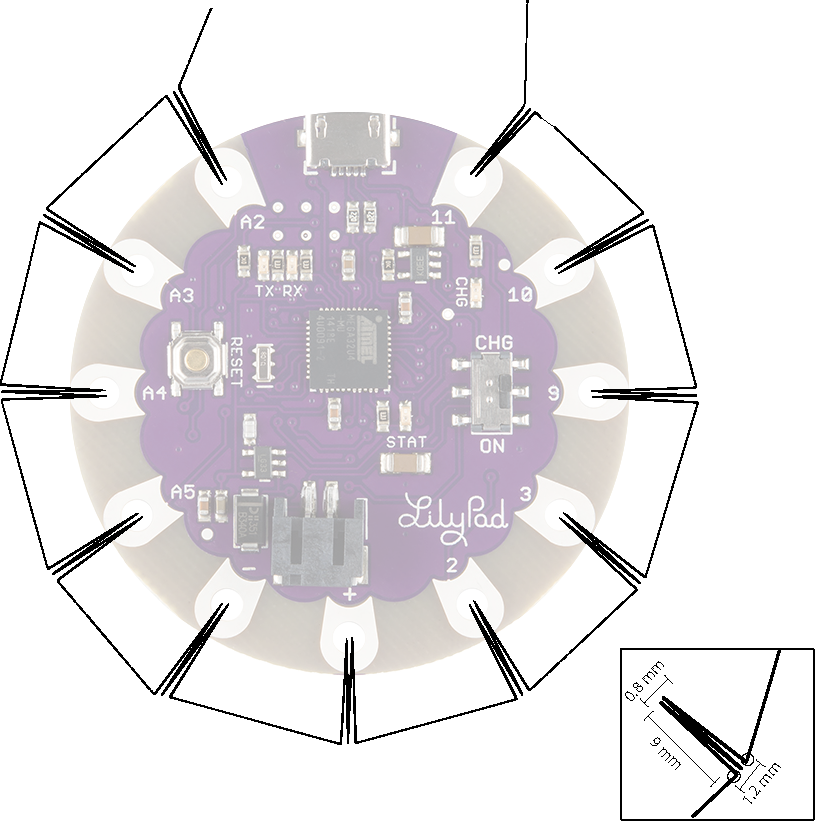
\includegraphics[width=0.8\columnwidth]{figures/LilyStitch}
  \caption{Embroidery pattern of LilyStitches for attaching LilyPad Arduino USB using an embroidery machine.}~\label{fig:LilyStitch}
  \vspace{-2em}
\end{figure}

The last technique uses the \textit{button sewing} presser foot in sewing machines. The user has to manually align each pin hole under the presser foot. While this requires some skill, it becomes efficient with practice. Of course, the user can also use the status-quo method of manually sewing into the holes using conductive thread \cite{Buechley:2008:LAU:1357054.1357123}. 
%And part stickers
The results of a sewing machine and manual sewing can be as reliable as using the embroidery machine, but they require more manual labor and time.


\subsection{Insulating circuit traces}
Insulating circuit traces, especially in wearable e-textiles, is paramount for their functionality. Textiles are flexible materials. Exposed traces may come in contact with each other as fabric folds or bends, creating shorts or undesired signals. Buechley et al.\ \cite{Buechley2009} proposed couching---stitching one thread over another---as a natural insulation technique for fabric circuit traces. However, they noted that sewing machines may leave gaps in the top stitch, making it an unreliable cover for the underlying conductive thread. Computer-controlled embroidery machines are much better at maintaining a consistent couching stitch, making them a perfect fit for this technique.


In Sketch\&Stitch, the draws circuit traces that she wants to insulate with her \textit{insulation color} marker. The system duplicates all objects in this color, and stores them in two design layers, the bottom layer in \textit{trace color} and the top layer in \textit{insulation color}. The layer colors are used to map to stitch types and to define the sequence of stitching layers in the embroidery software. 
%We describe this process further in Implementation section. 
While couching circuit traces has functional advantages, it has two pitfalls: It can have a pronounced visual impact on the design due to its thickness, and the build-up of stitches can reduce the flexibility of the base fabric, especially if applied to several traces in a small area.

\subsection{Handling Crossing Traces}
\begin{figure}
\centering
  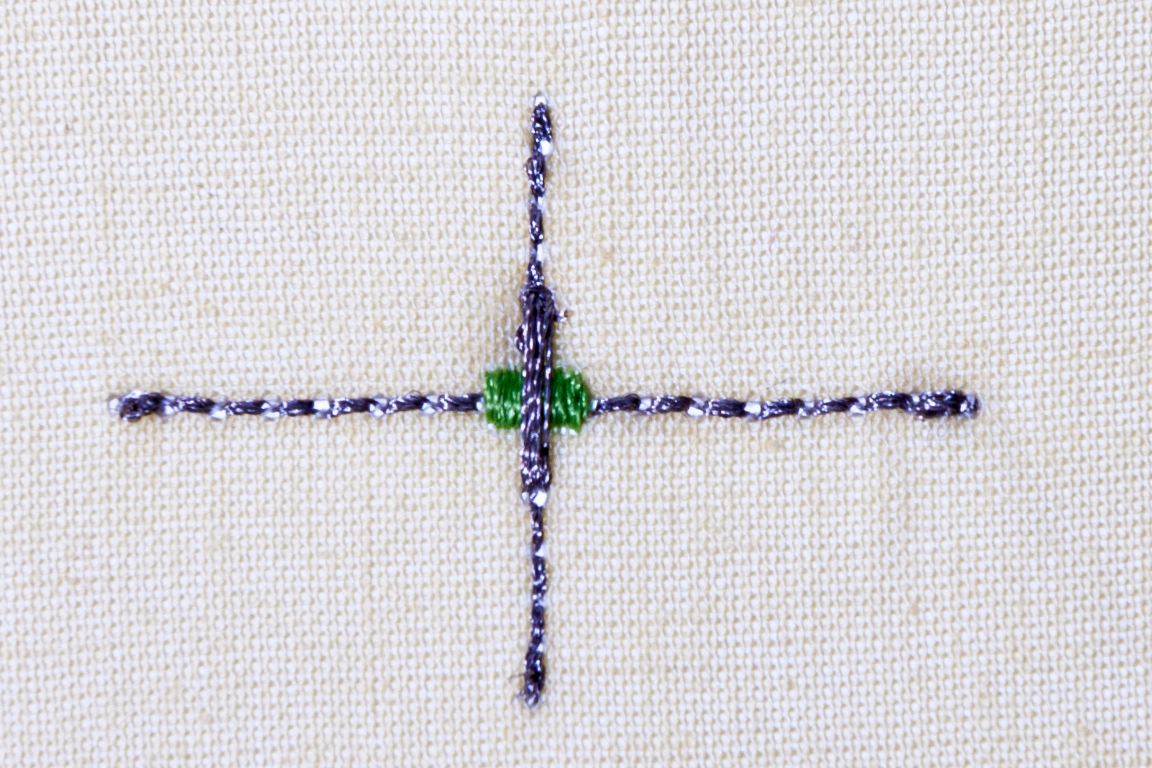
\includegraphics[width=1\columnwidth]{figures/BridgeStitch}
  \caption{Handling crossing traces: (a) shield sticker, (b) three layer embroidery design, (c) shielding using the BridgeStitch.}~\label{fig:BridgeStitch}
  \vspace{-1.5em}
\end{figure}

As the number of circuit elements increases in a design, the need for circuit traces crossing each other becomes inevitable. Dunne et al.\ \cite{Dunne:2012:MEC:2370216.2370348} manipulate the tension of the top and bottom threads to allow two conductive threads to cross without touching. However, from our experience, this technique does not provide fail-safe insulation, especially when pressure is applied to the intersection point. In addition, adjusting the thread tension to be too high or too low impairs the strength and appearance of stitches. It may also lead to ``thread birdnesting'', which causes the thread to tangle and the machine to stop.  
%various fabric-thread combinations require different tension settings and changing these settings may affect the appearance and strength of the stitches. 
Sketch\&Stitch instead provides users with the \textit{Shield Sticker}, an Embroidery Sticker to mark trace crossings to insulate on fabric. The user places the sticker over the intersection point and aligns the traces to its dotted lines (Fig.\ \ref{fig:BridgeStitch}.a). 
%Self crisscrosses of conductive thread are safe and do not need to be handled.
%This ensures that the bridge patterns with overlap with the traces. 


The rectangle in the Shield Sticker is used to locate it using color filtering and corner detection, and replace it with three design layers: the bottom layer contains a line segment for connecting one trace, the middle layer a line segment for insulating that trace, and the top layer an M shape to connect the perpendicular trace (Fig.\ \ref{fig:BridgeStitch}.b). The layers are colored to map to specific stitch types and sequence order in embroidery software. The top layer is mapped to a custom stitch pattern, the \textit{BridgeStitch} (Fig.\ \ref{fig:BridgeStitch}.c). It is similar to the LilyStitch but of consistent .8 mm width, and its tie-in and tie-off knots are on one end of the stitch each. The BridgeStitch is used to connect two separate segments (that can be up to 9 mm apart) without stitching between them.

%The layers are tinted in a color scheme that maps to specific stitches---triple running, zigzag 0.3/2.0, and a \textrit{bridge stitch}, respectively. And converted in embroidery software to a bridge embroidery pattern (Figure \ref{fig:BridgeStitch}).
%The bridge stitch, the top layer in the bridge pattern, is a single running stitch (9 mm long) stitched in an M shape. 

%3.7 mm





\subsection{Adding Interactivity}
% \begin{figure}
% \centering
%   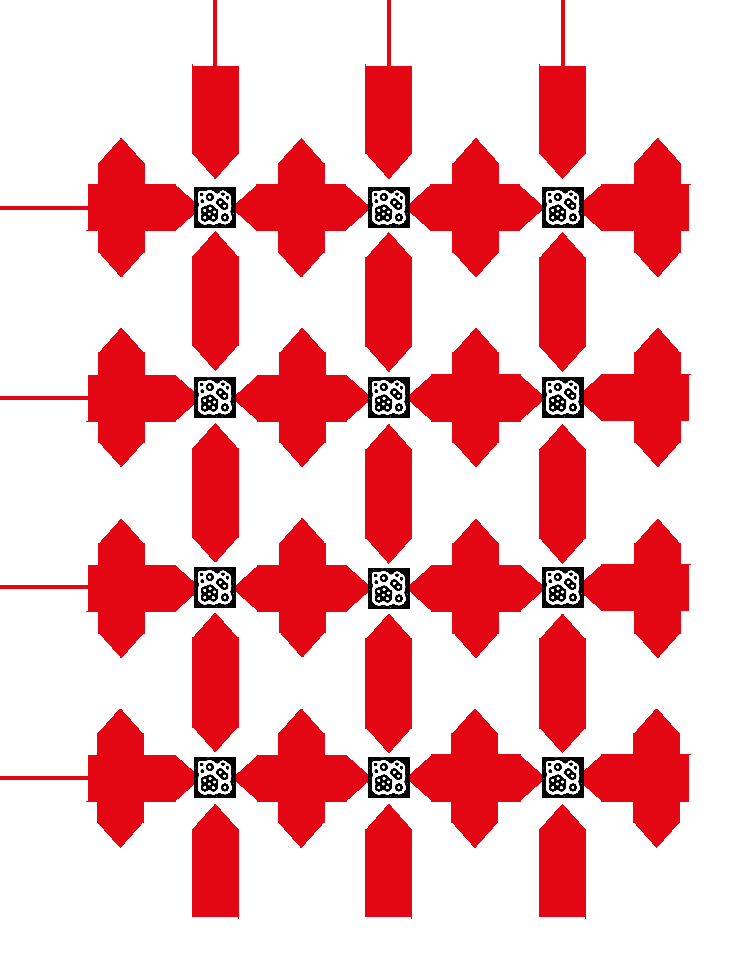
\includegraphics[width=0.6\columnwidth]{figures/RedStickers}
%   \caption{}~\label{fig:RedStickers}
%   \vspace{-2.5em}
% \end{figure}
Besides hardware electronics, users can use \textit{Sensor Stickers}, Embroidery Stickers to add touch sensors made from conductive thread directly onto the fabric. Sketch\&Stitch offers three such sensor types: a pushbutton, a slider, and a touchpad.
%actuators, e.g., by couching a shape memory alloy wire, and various touch sensors, as we will demonstrate in this section.

A capacitive pushbutton is the simplest sensor to create, by connecting any segment of conductive thread to a capacitive sensing circuit. The circuit can sense when the user's finger or body is in contact with the thread (touch) or not (no touch). Users can design pushbuttons to have a larger surface or an artistic shape by drawing and filling a shape with a \textit{trace color} marker. A resistive pushbutton can be created with two conductive traces 3--4 mm apart that the user bridges when touching, with one trace usually grounded, the other connected to an analog microcontroller input. Using this simple technique, users can create physical widgets of custom shapes, or convert artworks to touch-enabled surfaces, by using the \textit{trace color} marker to draw those parts of the art.

%When the user touches the two segments at the same time, a resistive sensing circuit registers a touch.

A slider can be implemented by placing several pushbuttons next to each other. A resistive circuit enables a slider with coarse resolution---the user bridges two neighboring buttons. A capacitive circuit can enable a higher resolution, by interpolating the position of a finger based on the amount of surface area it covers and its influence on neighbouring buttons.

% to determine more than one capacitive threshold for a single button. As the user's body comes in contact with more surface o with a capacitive sensor is interacted with by the user, the larger the capacitance will be. 

A matrix of such buttons, with each button connected to one IO pin, can be used as a 2D touchpad \cite{hamdan2016grabrics,5387040}. 
%offers the ability to detect all buttons being pressed at the same time, i.e., multi-touch. 
However, a 4$\times$4 touchpad would require 16 pins and traces. This complicates the wiring and may require additional hardware. Instead, using a layout of grid lines with time-multiplexing, as used in capacitive touchscreens, provides a sensor surface area capable of detecting individual touches, simple gestures, and sub-sensor point detection. It requires fewer pins ($4+4=8$ for a 4$\times$4 pad) and less power than scanning individual buttons. 
%However, it cannot support multi-touch. A grid layout can be connected to a capaciiuve or resistive circuit. But due to the low resistivity of the human finger, not all hardware can detect a direct touch. One alternative is to use pinching as an input technique. Hamdan et al. [] were able to detect the location and angle of a pinch on a matrix of resistive textile buttons using simple machine learning algorithms.
Based on design recommendations from Texas Instruments for capacitive touch sensing with their MSP430 microcontroller\footnote{ www.ti.com/lit/an/slaa363a/slaa363a.pdf}, we designed an embroidery pattern for a touchpad sensor. Similar to the \textit{Shield Sticker}, the \textit{Sensor Sticker} has rectangles at the intersection points of the grid. The system detects these rectangles and replaces the area with a grid in the same three-layer design. The sensor grid uses the \textit{trace color} and is otherwise treated similarly to hand-sketched circuit traces.

\begin{figure}
\centering
  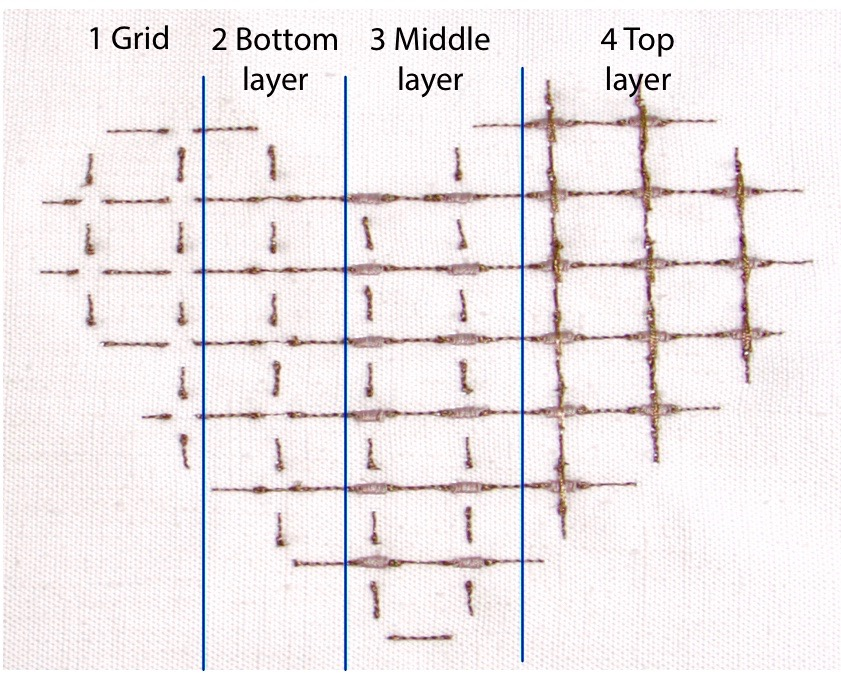
\includegraphics[width=0.7\columnwidth]{figures/heart}
  \caption{Sensor sticker cut into a heart shape and embroidered to show the three design layer.}~\label{fig:Sensor}
  \vspace{-2.5em}
  \end{figure}
  
To create a sensor in Sketch\&Stitch, the user prints the \textit{Sensor Sticker} on a sheet of adhesive paper, cuts it into the desired shape to create a slider or a touchpad, and sticks it onto the fabric, then draws connecting traces from two sensor grid edges to pins of a controller using the \textit{trace color} marker. After capturing the design, the user removes the \textit{Sensor Sticker}, and the embroidery machine stitches the sensor pattern in place. Fig.\ \ref{fig:Sensor} shows a 2D touchpad at different stages of the embroidery process to show the different layers.

Electronically speaking, rectangular sensors are the easiest to create that way. The user connects to them at two of their adjacent edges. Other convex shapes require per-line calibration in software to account for the different lengths of grid lines, and concave shapes may also require multiple connections per line if it is interrupted, like the top row in Fig.\ \ref{fig:Sensor}.
%The grid was designed based on the recommendation of Texas Instruments 


% constructed by “opening up” a capacitor structure so that the
% electric field can be interfered with by a conductive foreign object, in this case, a fingerWhen a conductor, e.g., a finger,
% comes into the area above the open capacitor, the electric field is interfered with causing the
% resulting capacitance to change. The coupling of the conductive finger into the capacitive sensor
% increases the capacitance of the structure beyond the baseline capacitance, the capacitance of
% the sensor with no touch. By continuously measuring the capacitance of the sensor(s) in the
% system and comparing each result to a predetermined baseline capacitance, the system
% microcontroller can determine not only on/off button functions for each sensor element but also
% “amount” of press used for more complex interfaces such as positional sliders. 
% The base capacitance of such a design is affected by stray capacitances on the PCB as well as
% potentially other environmental effects such as temperature and humidity. Therefore, the
% detection system needs to constantly monitor and track this variation for correct comparison to
% touch events. 



 

\subsection{Concealing Traces and Components}
Our system offers four strategies to conceal circuit traces and hardware components in a design: the first is drawing circuit traces to be part of the artwork. The second is drawing circuit traces close to art outlines. 
%The spacing constraint of 2.5 mm need not to be applied between conductive and non-conductive threads. 
While this strategy does not hide the traces, it makes them less obvious. 
%since the width of art stitches is relatively larger than trace stitches.
The third strategy is camouflaging traces by insulating them with a thread color that matches the color of the base fabric \cite{Buechley2009}. Traces will not be hidden completely, but depending on the desired application, this technique may be sufficient to occlude electrical connections. 

The fourth strategy allows users to hide fabric circuits and hardware components completely. It uses two layers of fabric: a top layer for sketching the artwork, and a bottom layer for sketching circuit traces and adding Circuit Stickers. The two fabrics are captured and embroidered individually. At the end of embroidery, the user attaches components to the bottom fabric and manually layers the fabrics on top of each other. Touch sensors will work through a thin top fabric. For components that need to be visible on the surface, such as light sensors and LEDs, the user may cut openings into the top fabric. Another option is attach these parts on the top fabric and use one of the suggested thread-based attachment techniques to connect them to their contact surface on the bottom layer. This technique can also be used to create multi-layer textile circuits \cite{Dunne:2012:MEC:2370216.2370348, 5387040}, with the addition if an insulator like non-conductive fabric, between any two conductive layers. 







\section{Walkthrough: Interactive Flower}


We illustrate Sketch\&Stitch's basic design pipeline using the example of an interactive flower that emits light patterns when the user touches one of its leaves. The flower includes 3 LEDs, 1 touch sensor, 1 battery holder, and 1 microcontroller 
%ATmega32U4 Board 
from the LilyPad kit. Fig.\ \ref{fig:Walkthrough} shows the design pipeline.

\begin{figure} 
\centering
  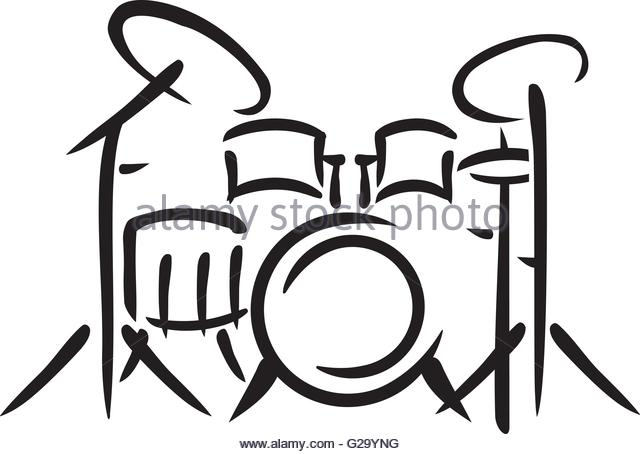
\includegraphics[width=0.9\columnwidth]{figures/Walkthrough}
  \caption{Sketch\&Stitch interaction walkthrough.}~\label{fig:Walkthrough}
  \vspace{-1.5em}
\end{figure}

\subsubsection{Sketching and Placing Circuit Stickers}
At the beginning, the user hoops her fabric and calibrates her marker color palette using the Sketch\&Stitch printed template and smartphone app.
%She places her fabric and markers under the camera mount, and presses  
%prints Circuit Stickers on adhesive paper using her home printer. She cuts the stickers she need for the project---board and pixels. Then, she frames the center of a T-shirt in an embroidery hoop. 
Using a violet \textit{art color} marker, she starts drawing the outline of a flower (\ref{fig:Walkthrough}a). She then places Circuit Stickers inside the flower to estimate their size and location (\ref{fig:Walkthrough}b). Once satisfied with the arrangement, she peels off the stickers' backing and attaches them to the fabric. Using the pink \textit{trace color} marker, she draws circuit traces between the Component Stickers (\ref{fig:Walkthrough}c). She also draws a trace from a pinhole on the controller to the leaf of the flower to create a simple capacitive pushbutton. If she makes a mistake while sketching, she pads a damp cloth on the fabric to erase it.

\subsubsection{Capturing and Embroidering Design}
When she is ready to embroider her design, she presses the button next to the camera mount, and the system captures a picture of the design inside the hoop (\ref{fig:Walkthrough}d). She then secures the hoop in the embroidery machine and uses the embedded display to review the digital embroidery patterns of her design---art and circuit patterns. Since there are no \textit{Embroidery Stickers} to remove in this design, she threads the embroidery needle with conductive thread and starts the embroidery (\ref{fig:Walkthrough}e).  The machine begins embroidering the circuit pattern automatically. Once it is done, it prompts her to change threads. The user picks a non-conductive thread of the color she wants for each part (red for the flower, green for the leave and stem outlines) and starts the machine again. 

% \subsubsection{Debugging}
% After embroidery, the user removes the hoop from the machine, and trims jump stitches. She places the board and pixels over the fabric to verify the alignment of their pins and contact surface. She uses a digital multi-meter to test her traces for any shorts or undesired connections. 

% \subsubsection{Designing Incrementally}
% She cuts a sensor sticker (3$\times$4), and adheres it on fabric. She draws traces from the sensor to the board. Switching to the purple marker, she completes the design of the mandala. She take a picture of the new design, removes the sensor sticker, secures the hoop in the machine, and starts the embroidery machine stitching the sensor and remainder artwork. 

\subsubsection{Attaching Electronics}
After embroidery is complete, the user removes the hoop from the machine, and trims jump stitches using a scissor. She cuts and peels a piece of Z-tape and applies it on the back of her hardware components. Guided by the Circuit Stickers, she determines the location and orientation of each component. She removes the stickers and attaches the matching components to the fabric aligned to their contact surface (\ref{fig:Walkthrough}f). Finally, she inserts a battery into the battery holder and sees her design augmented with a touch-sensitive lightup effect.




%become Finally, the user uses, e.g., Arduino IDE, to program the functionality of her e-textile.



%The user is free to perform this step in any environment since her input is not tracked in real-time. 

\subfile{Implementation}


\section{Technical Considerations: Embroidering with Conductive Thread}

We use a Bernina 880B
%\footnote{www.bernina.com/880}
embroidery machine and its software, DesignerPlus v.8, with Shieldex 117/17 dtex 2-ply silver sewing thread (linear resistance < 30 $\Omega$/cm). 
%http://www.shieldextrading.net/products/yarns-threads/
This thread can carry current for power and signals. The embroidery machine requires two types of thread: a top thread that appears on the surface of the fabric, and a bobbin thread that runs on the back side of the fabric to pull the top thread down. We use conductive thread as a top, or fashion, thread. Embroidery machines give users more control over the shape of the top thread compared to the bobbin. For conductive thread, we set the stitching speed to 300 stitch/min to reduce the heat and friction that is associated with high speeds, and used a light weight bobbin thread (60 wt). Embroidery is one of the most stressful textile processes for conductive thread \cite{5387040}. This stress leads to thread breaks, which can lead to discontinuities in circuit traces. We were able to minimize breakage by reducing stitching speed. To understand how best to embroider conductive thread, we performed a battery of experiments.

\paragraph{Resisitivity}
 \begin{figure}
\centering
  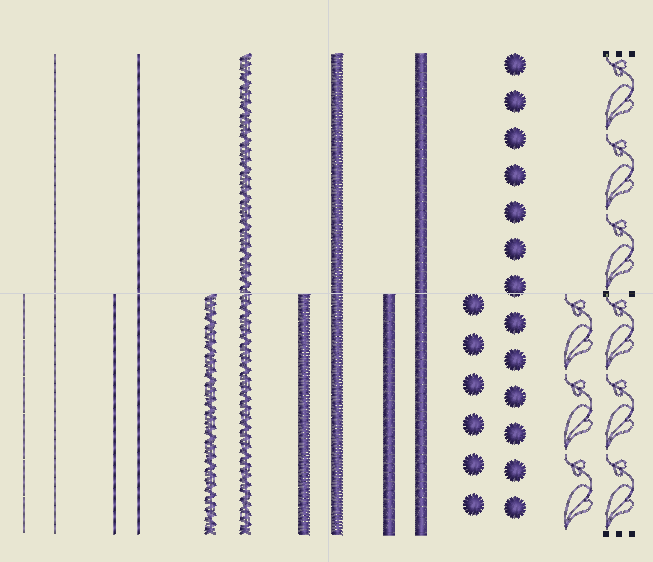
\includegraphics[width=1\columnwidth]{figures/Resistance}
  \caption{Resistance test: resistance measurements of conductive thread traces using different stitch variants in 5 and 10 cm segments.}~\label{fig:Resistance}
  \vspace{-0.5em}
\end{figure}
We first tested the effect of stitch type on the resistance of circuit traces. Unlike traditional copper wire, conductive thread has a relatively high resistance, which plays a key role when laying out fabric circuits. It means that longer traces drop significantly more voltage, consuming power and limiting the amount of current that can be delivered to components. Increasing the number of connections between the conductive fibers that compose a thread, by choosing different stitch types such as running, zigzag, or satin, can lower its resistance (Fig.\  \ref{fig:Resistance}). Of these, we found a zigzag stitch with 2 mm spacing to be the best trade-off of resistance and density, i.e., stiffness, but harder to insulate. In Sketch\&Stitch we use triple running stitch for narrow and insulated traces, and zigzag (2 mm spacing) for wider trace lines. 

\paragraph{Spacing}
Next, we tested the minimum required spacing between adjunct exposed traces to avoid undesired connections. We measured for continuity just after embroidery, and after one and two weeks of frequent fabric handling. Fraying fibers connected traces at 1.0 and 1.5 mm spacings. Tie-in and tie-off knots, which are often wider than the trace itself, created undesired contacts on the back of fabric. We conclude that a 2.5 mm is the safe minimum distance between exposed traces.
%  \begin{figure}
% \centering
%   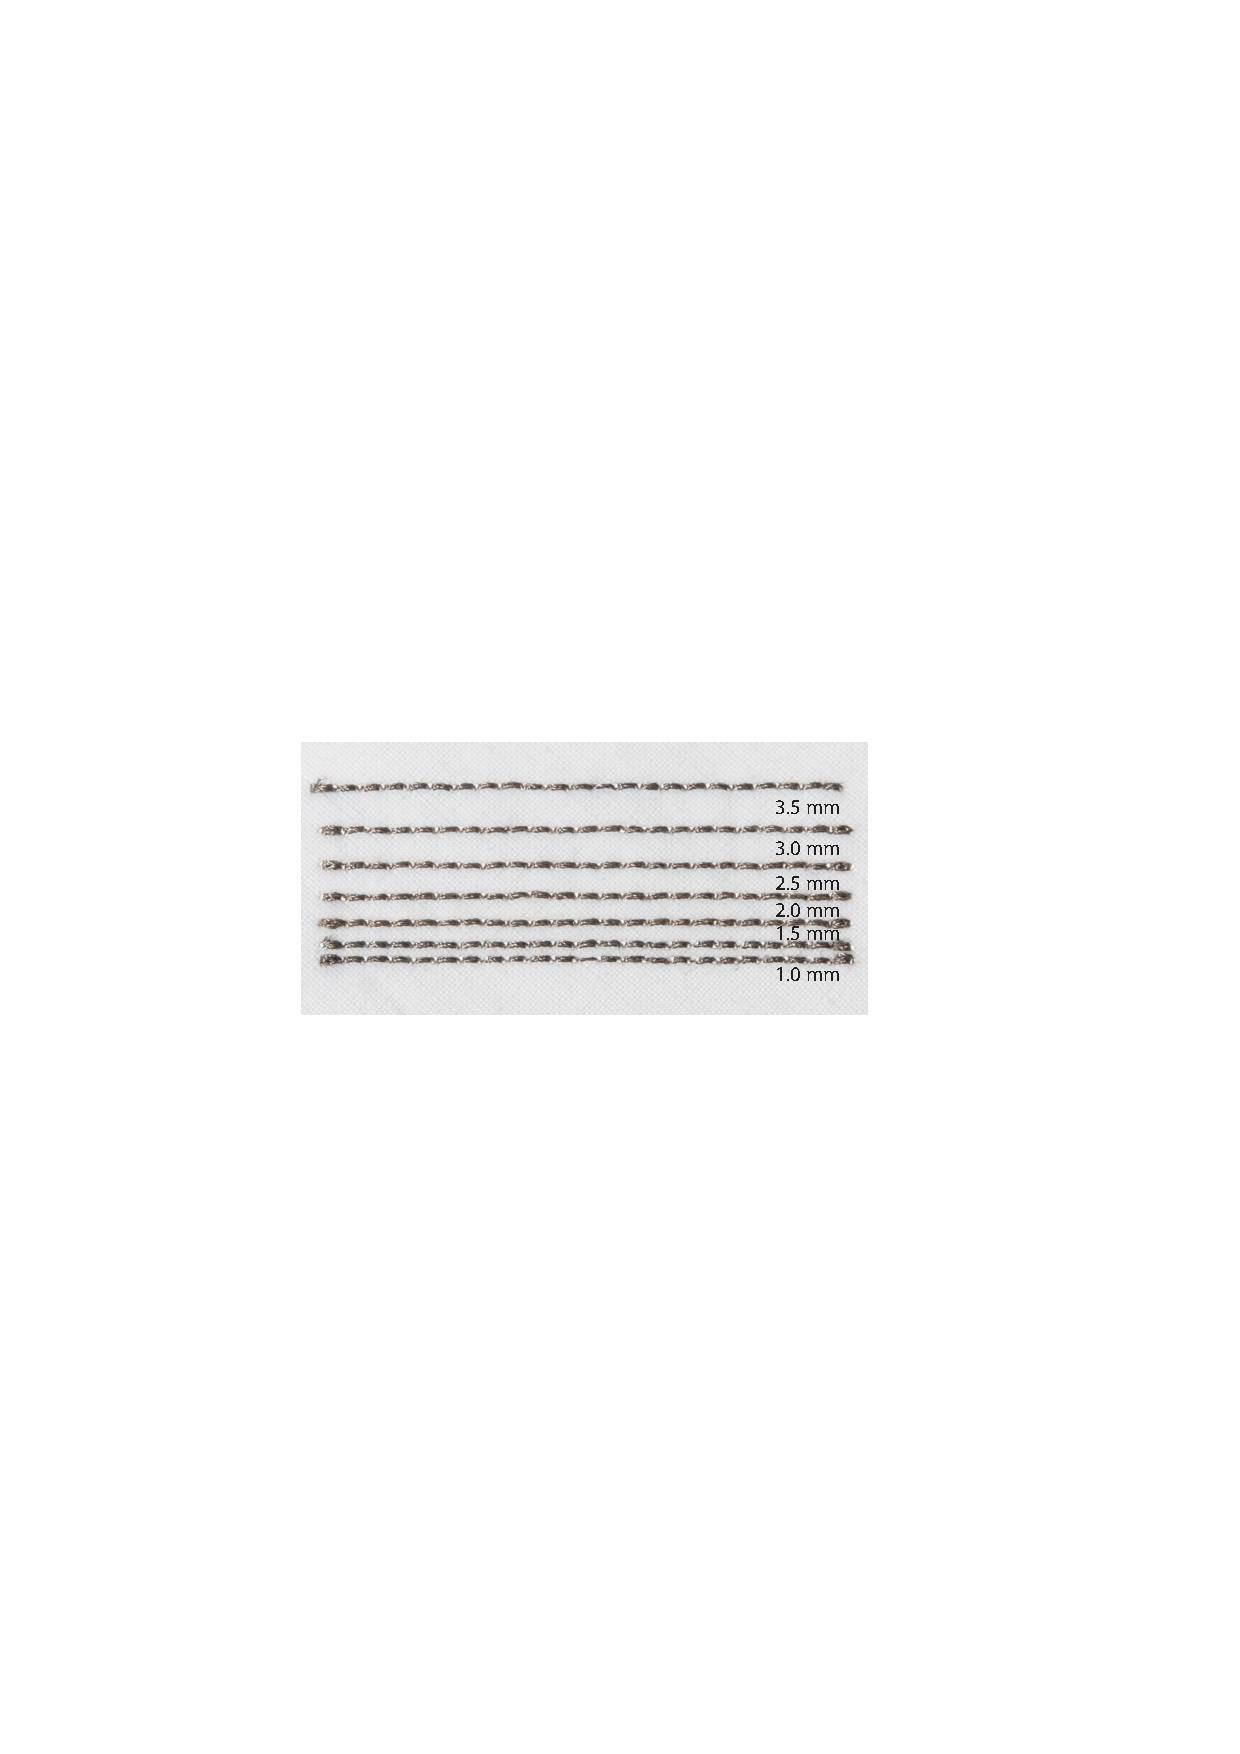
\includegraphics[width=0.8\columnwidth]{figures/Spacing}
%   \caption{Spacing test: electrical connection measurements of exposed conductive thread traces spaced at 1.0 mm - 3.5 mm apart.}~\label{fig:Spacing}
%   \vspace{-1em}
% \end{figure}


\paragraph{Insulation}
\begin{figure}
\centering
  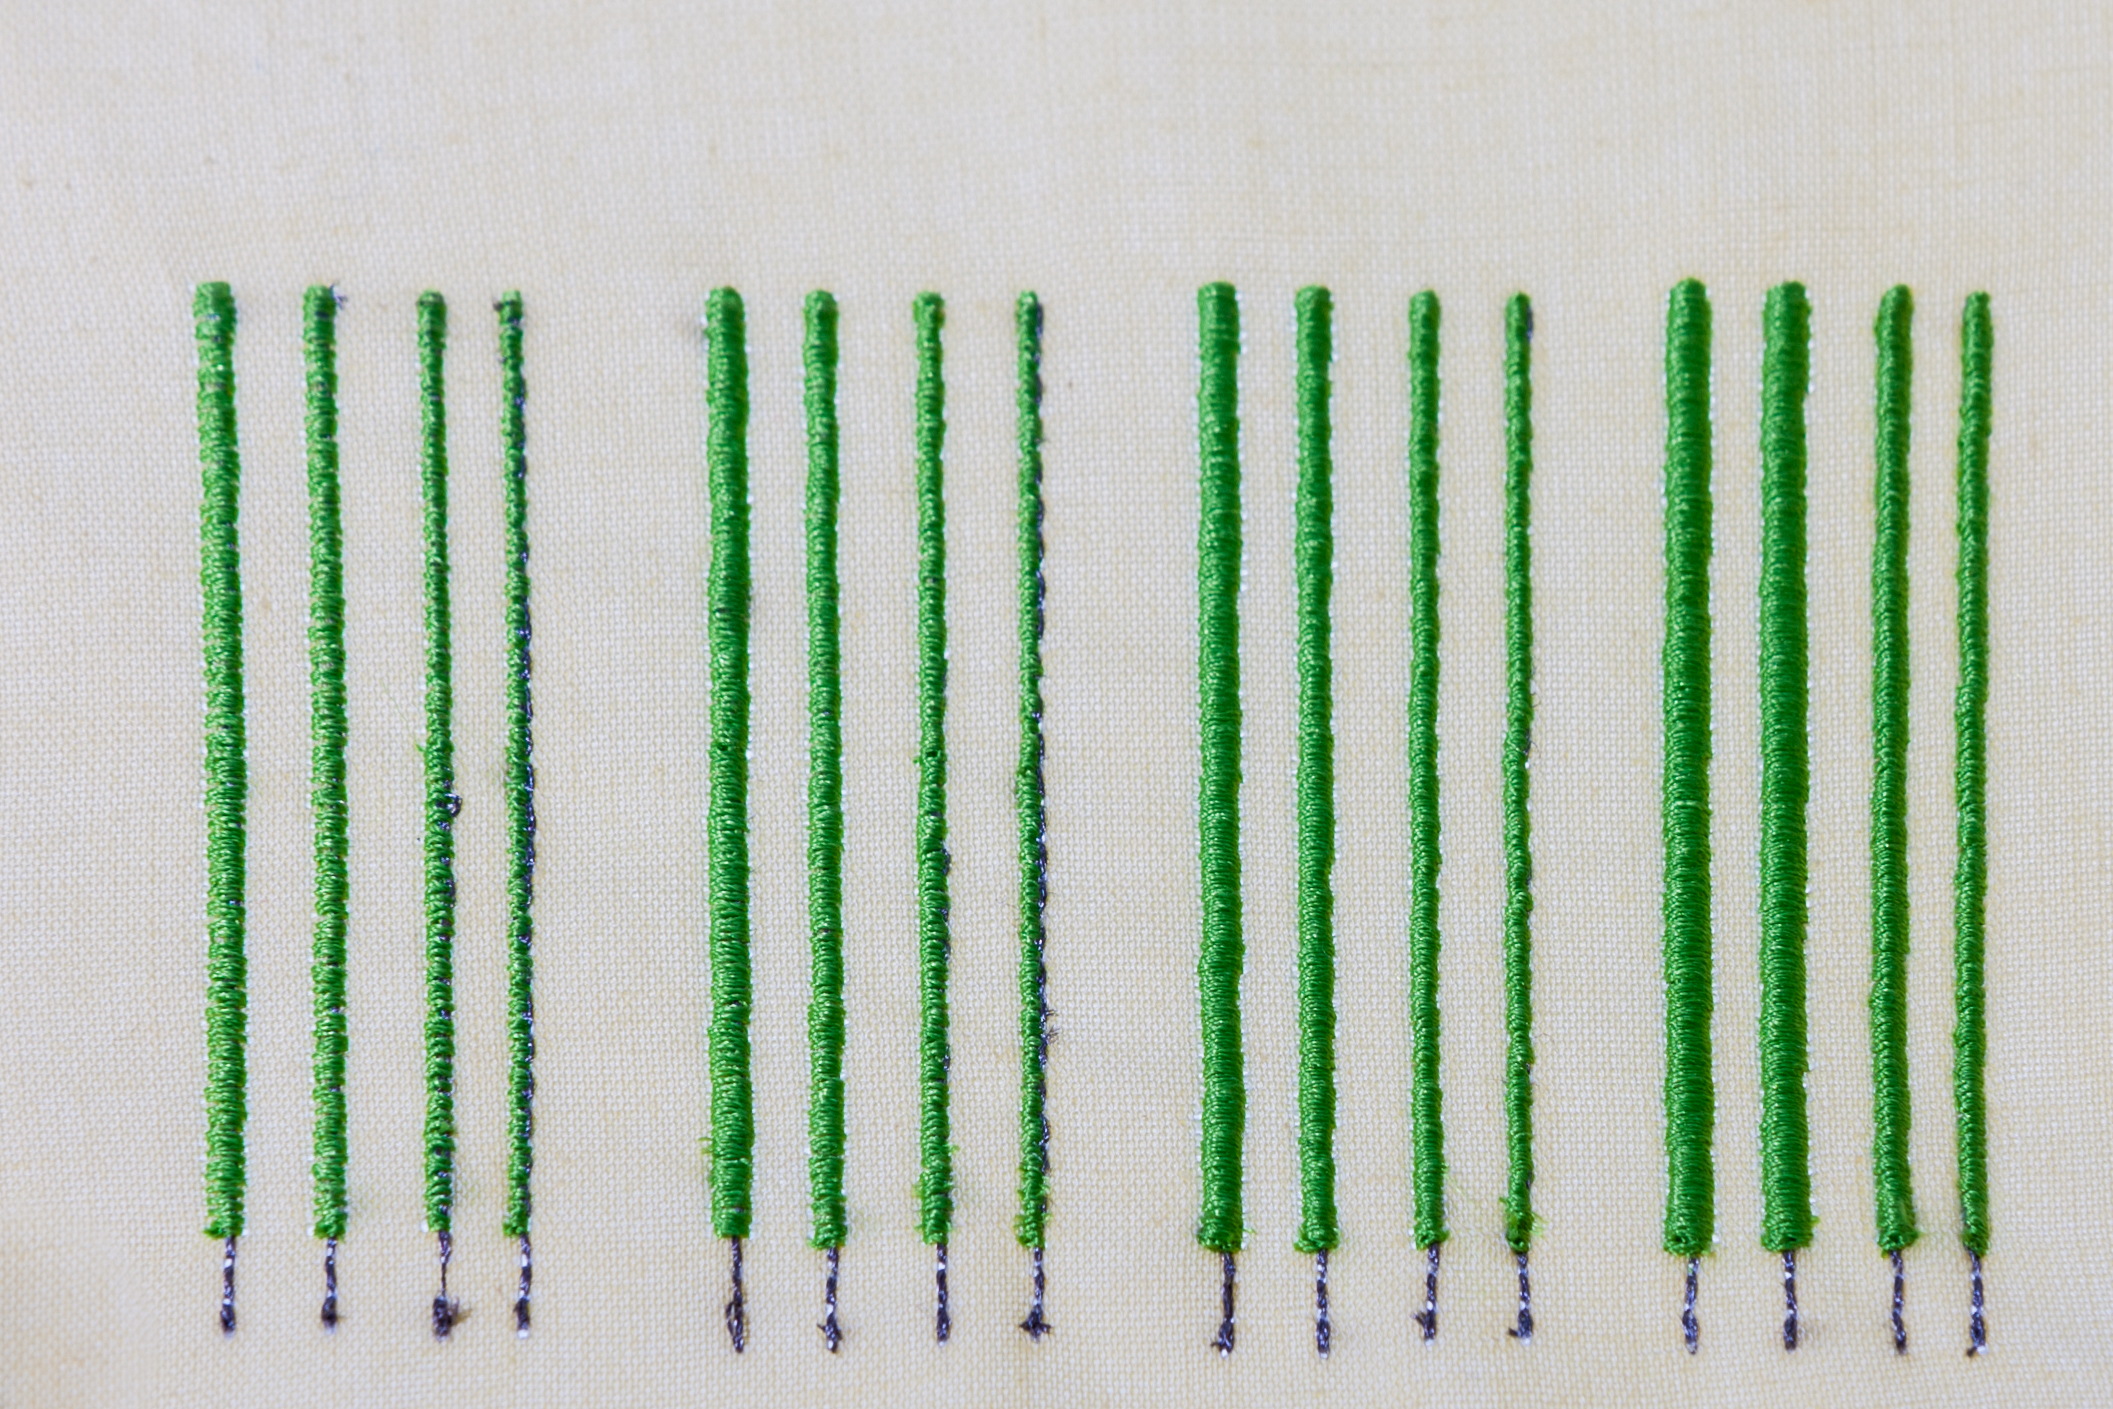
\includegraphics[width=1\columnwidth]{figures/Insulation}
  \caption{Insulation test: electrical connection measurements of a zigzag insulation stitch of different stitch widths and spacings when pressed against exposed traces of conductive thread.}~\label{fig:Insulation}
  \vspace{-2em}
\end{figure}
Finally, we evaluated insulation stitches that can cover and prevent circuit traces from creating electrical connections even if they come in direct contact with each other.

The zigzag stitch (a back-and-forth stitch) is the most common for couching, stitching one thread over another. It is defined by two main parameters: width and density, or spacing between threads. We manipulated these to find a good stitch to insulate circuit traces. 
%Insulating conductive thread is challenging due to its fraying properties. 
Again, we looked for a trade-off between the reliability of the insulation and the width and density of the stitch. A wider insulation dictates the smallest distance between adjunct traces and may impact the visual design. A dense insulation stitch can reduce the flexibility of underlying fabric, especially if applied to several traces in a small area.

Fig.\ \ref{fig:Insulation} illustrates the parameters tested and summarizes the results.
We laid the insulated traces on top of non-insulated conductive traces, and applied four amounts of pressure (1, 5, 15, 30 N) at 5 equidistant points along each trace. An insulation stitch of 1.5 mm width and .3 mm spacing best satisfied our technical and design requirements. It also insulated conductive traces on the wrong side of the fabric. Based on this result, two insulated traces can be spaced as closely as 2 mm---closer than uninsulated ones.




\section{Example Applications and Emerging Design processes}
We invited a hobbyist artist with a technical background (female, 24 years old) to use and evaluate the design pipeline of Sketch\&Stitch over three days. After we described the system to her, she developed the three e-textile projects below. At the end of the third day, we interviewed her to understand the design process that emerged while using our system. We describe these processes after the examples.


\subsection{Wearable Mandala}
\begin{figure} [h!]
\centering
  \includegraphics[width=1.1\columnwidth]{figures/Mandala} 
  \caption{Example 1: The Wearable Mandala. Size 150$\times$150 mm, 20,000 stitches, 4 color changes, stitch duration 28 minutes.}~\label{fig:Mandala}
  \vspace{-0.5em}
\end{figure}
The first example is a wearable application. The artist augmented a finished cotton t-shirt with 8 LEDs, a microcontroller, and a hidden battery. The mandala lit up every time she received a message on her smartphone. The artist used the outlines of the mandala to conceal circuit traces and integrate them as part of the artwork (first concealing strategy). She embroidered frames to house the hardware components, and a contact surface for the battery holder. The battery holder was attached to the contact surface from the wrong side of the fabric to hide it.



\subsection{Interactive Desk Mat}
\begin{figure} [h!]
\centering
  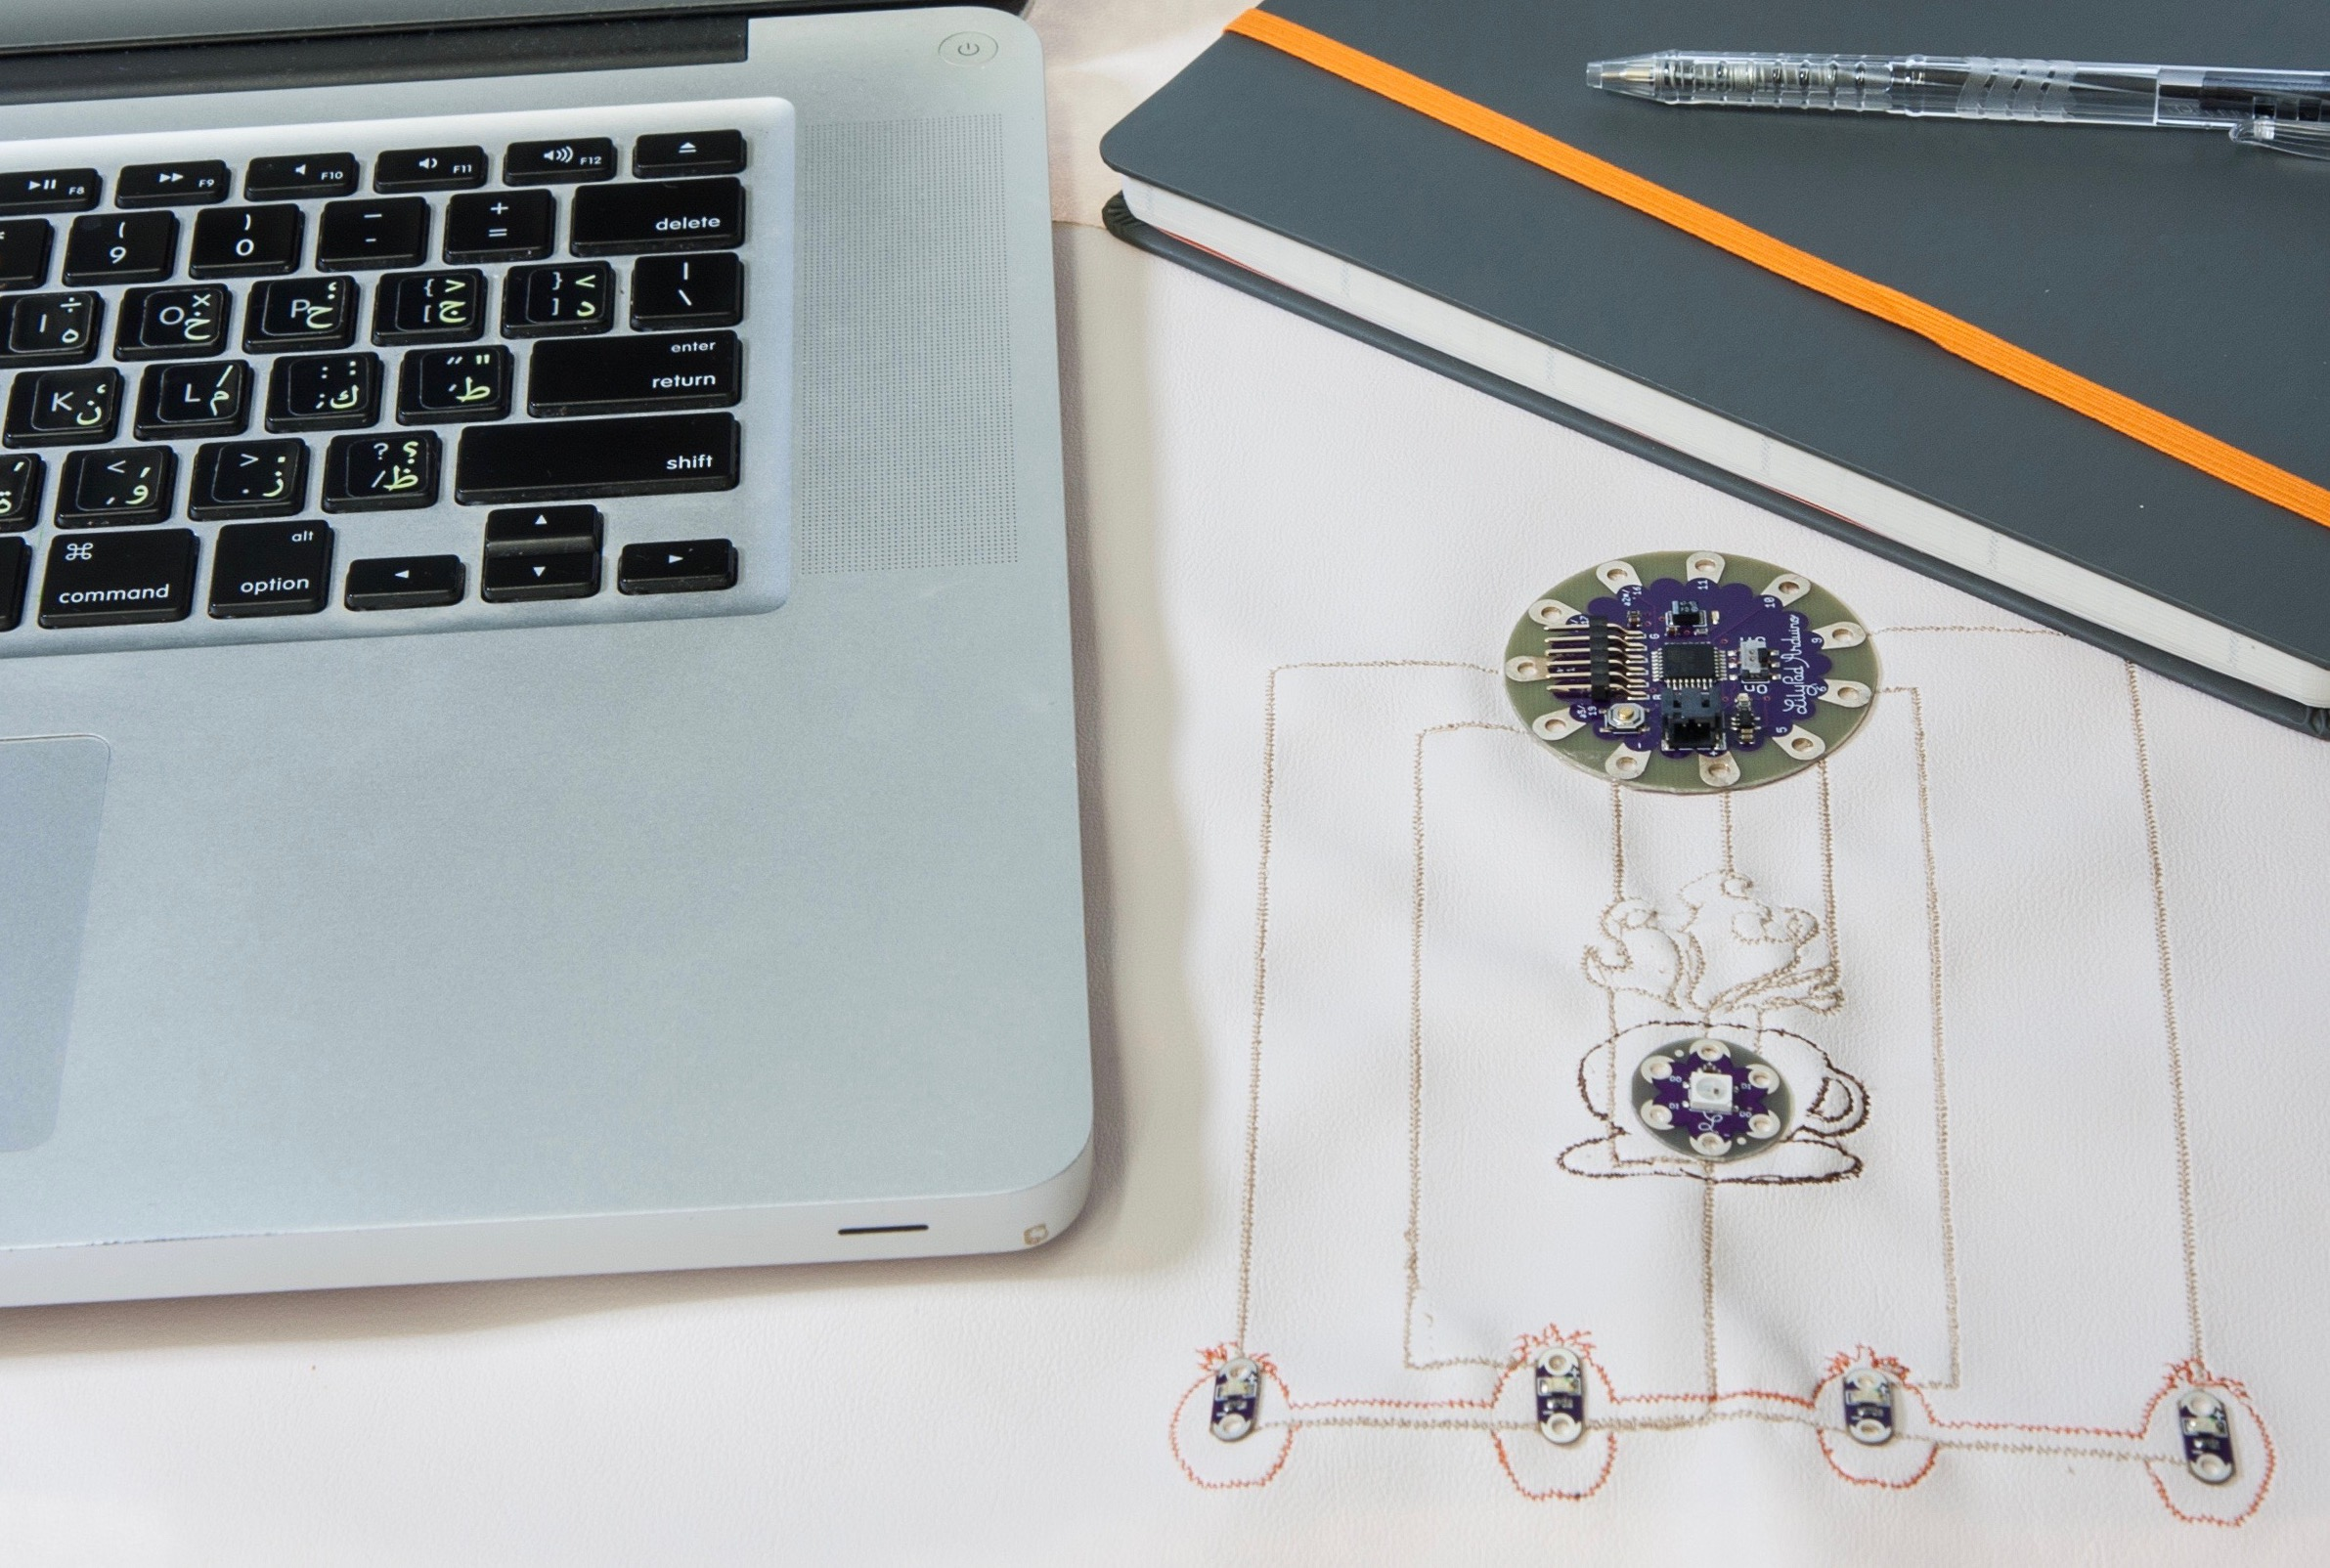
\includegraphics[width=1\columnwidth]{figures/DeskMat}
  \caption{Example 2: The Interactive Desk Mat. Size 160$\times$130 mm, 9,000 stitches, 3 color changes, stitch duration 13 minutes.}~\label{fig:DeskMat}
  \vspace{-1.5em}
\end{figure}
The second example is an interactive leather desk mat. The artist designed an interface for the ``Pomodoro'' time management technique, using 4 LEDs, a pixel board, and a controller. She plugged the controller into her computer to power it. A timer was programmed to light up an LED every 25 mins to indicate the start of a work interval. Between each work interval, the pixel board flashed to announce a 5 min break. Once all 4 LEDs were lit up, the pixel board lit up to announce a longer break. In her design, the artist used a ruler to draw straight circuit traces for the LEDs. Technical lines seemed appropriate for the context of this application. She drew steam coming out of the coffee cup and used it to connect traces at the center of her artwork. 


\subsection{One-Hour Nap Pillow}
\begin{figure} [h!]
\centering
  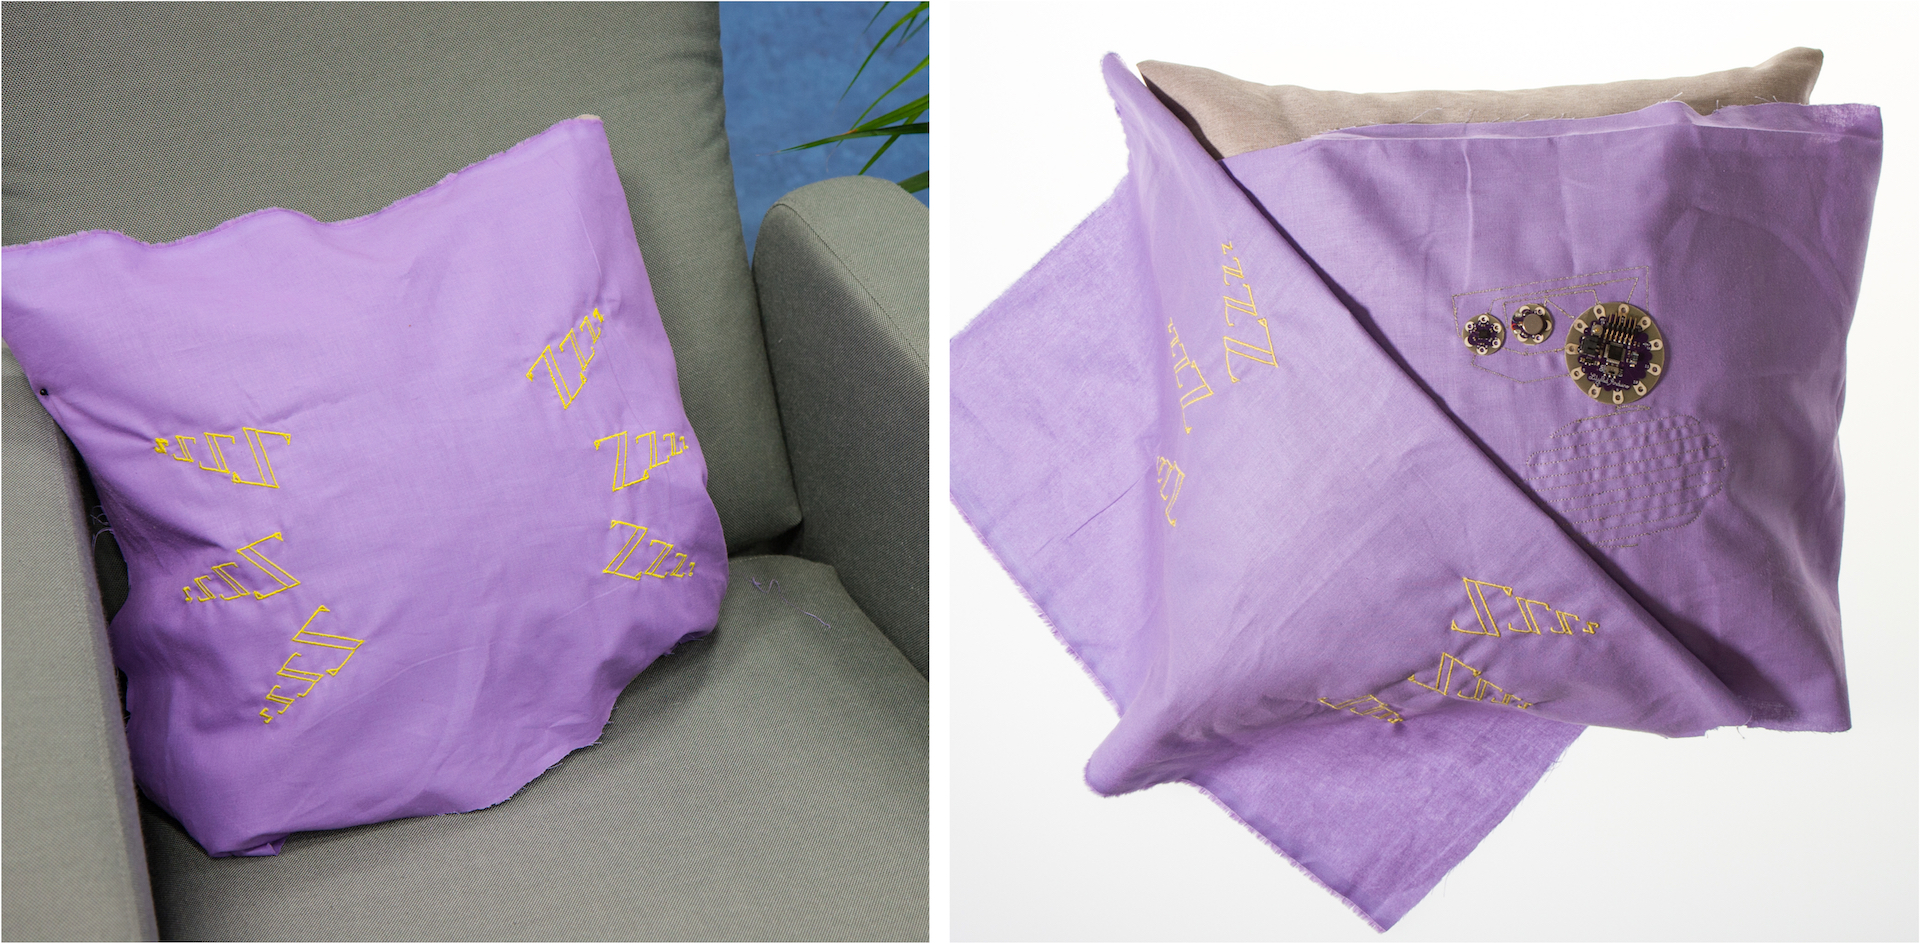
\includegraphics[width=1\columnwidth]{figures/Pillow}
  \caption{Example 3: The One-Hour Nap Pillow. 16,000 stitches, 2 color changes, stitch duration 23 minutes}~\label{fig:Pillow}
  \vspace{-0.5em}
\end{figure}
The one-hour nap pillow contains a touch sensor that detects when a person first puts their head on the pillow, and awakens him gradually using different vibration patterns after one hour of continuous contact. The user can snooze the pillow by shaking it. An accelerometer signals a 5- or 10-minute snooze based on shaking intensity. The pillow consists of two fabric layers: the lower layer contains the touch sensor and circuit, and the top layer is embroidered with a simple artwork. Our user sketched the artwork on one side of the pillow case. She then used the machine's embedded display to mirror and stitch the pattern also onto the other side. 


\subsection{Emerging Design Process}
\textit{Doodle on paper and commit on fabric}. The artist always started sketching her ideas on paper. She did not perceive fabric as a medium for doodling. Even with undo capabilities, she was hesitant to ``waste a good piece of fabric''. She also used Circuit Stickers on paper and routed traces near art contours. Once she developed her design idea, she copied her design onto fabric. However, she reported that working on fabric still allowed her to visualize the final product better, and sometimes made her make changes to her original design, e.g., strategically repositioning Circuit Stickers on a shirt to convey the design idea.

\textit{Sketch to fit a circuit.} In one of her projects, the artist printed a design inspiration she found online and used it to sketch her circuit. She placed Circuit Stickers on the printed paper and drew traces following design contours. Once she was satisfied with the circuit, she started to sketch her version of the design on fabric with the adaptations. She reported that this technique allowed her to sketch an artwork that fits a circuit instead of fitting a circuit into a design.

\textit{Integrate or hide.} The artist noted that sometimes she was able to incorporate circuit traces in her design but not circuit boards and components, and sometimes the reverse. Sketch\&Stitch supports both situations using the layered fabric technique to hide parts of the circuit.


\section{Limitations and Future work}

Sketch\&Stitch has several important limitations. Since the system depends on a color scheme to process and recognize the user's sketch, users are limited to a range of distinguishable marker colors (their choice of thread colors is only affected if they stitch in iterations.)
In addition, the system can only recognize sketches on fabric of solid colors. Drawings on patterned and dark fabrics are very challenging to capture.  
Drawing on textured fabric can lead to path discontinuities and variations in sketch colors due to change in pressure applied to the marker. For these materials, gestural interaction and projection-based feedback may be beneficial. Finally, the system supports two types of stitches---one for filling and one for lines and outlines. Tool proxies with design constraints \cite{mueller2012interactive} could be used to define other stitch types.


As Sketch\&Stitch automates the conversion of freehand sketches to embroidery patterns, jump stitches are very frequent and require trimming to avoid short circuits. High-end embroidery machines offer automatic trimming with a penalty of increased embroidery time. For fewer jump stitches, we could reorder the embroidery sequence of individual stitch objects algorithmically.

Finally, the current version of Sketch\&Stitch does not offer the autorouting and design rule checks for fabric circuits known from PCB layout tools. While users can test their circuit early and frequently in the design process, we believe that embroidery should offer an opportunity for circuit design and validation. Eichinger et al.\ \cite{eichinger2007using} presented early work on using PCB layout software (Eagle) to create embroidered fabric circuits. 
%However, they targeted people who are familiar with PCB layout software.
In future work, we would like to examine how to auto-route circuit traces based on the outlines of the artwork, inspired by \cite{savage2014series}.

%Our capture system cannot distinguish between overlapping lines in a single connection and between two connection.

%The camera capture setup should be well lit to avoid noise from shadows and inconsistent light. 

%In this paper we mainly focused on LilyPad electronics kit. Sketch\&Stitch ca support any off-the-shelf electronics, including DIP and SMD packages, as long as they have a 2.5 mm pitch between leads.
%%trade off between reliable contact surface and smaller contact points.

%The next step for conductive embroidery is to examine using the conductive bobbin thread together with conductive top thread to create multi-layer electrical devices.  

%Ultimately an embroidery machine can be adapted to work like a pick and place machine---placing and stitching electronic components on fabric based on design file. 


\section{Conclusion}
This paper described Sketch\&Stitch, a proof-of-concept system for fabricating e-textiles. The system combines physical sketching with a computerized embroidery machine offering users the benefits of direct making and the power of digital tools. The system is targeted at artists, designers, and makers especially during the early stages of e-textile design. We demonstrated the advantages of our design pipeline.


Particular advantages of embroidery machines for e-textile fabrication are that (a) they produce very accurate and consistent stitches over a relatively large surface, (b) their speed, (c) embroidery patterns of circuit elements such as sensors, passive components, antennas, etc., can be pre-programmed, modified, shared, and reused, always providing consistent results, (d) they can be programmed to automatically shield circuit traces, (e) embroidery is an additive manufacturing process that can be use on tailored and finished textiles, 
%reduces the waist created from e-textile fabrication, 
and finally (f) they are accessible to end users.


%more agency and control over the final outcome \cite{}
% BALANCE COLUMNS
\balance{}

% REFERENCES FORMAT
% References must be the same font size as other body text.
\bibliographystyle{SIGCHI-Reference-Format}
\bibliography{sample}

\end{document}
%%% Local Variables:
%%% mode: latex
%%% TeX-master: t
%%% End:
